% The Thaumaturgy and Necromancy supplement for Sanguine Dreams
% Organized and largely written by Poetics

\documentclass[10pt,twoside]{extarticle}

\usepackage{pdfpages}
\usepackage{multirow}
\usepackage{bookman}
\usepackage{wallpaper}
\usepackage{color}				% allows color
\usepackage{pifont}				% Special symbol library
\usepackage[usenames]{xcolor}	% Add coloration if necessary
\usepackage{enumitem}
\usepackage{tocloft}
\usepackage{titlesec}
\usepackage{fancyhdr}		% Custom headers/footers
\usepackage[normalem]{ulem}

% This is to offset the "two-side" option above,
% required for the FancyFooter package to work
\setlength{\oddsidemargin}{0.87in}
\setlength{\evensidemargin}{0.87in}

\pagestyle{fancy}
\fancyhead{}
\renewcommand{\headrulewidth}{0pt}
\fancyfoot{}
\fancyfoot[CE,CO]{\sc{Ch.} \leftmark}
\fancyfoot[LE,RO]{\thepage}
	
% All for the TOC
\renewcommand{\cftsecleader}{\cftdotfill{\cftsecdotsep}}
\renewcommand\cftsecdotsep{\cftdot}
\renewcommand{\contentsname}{Table of Contents}
\cftsetindents{section}{0in}{0.25in}
\cftsetindents{subsection}{0.25in}{0.31in}

\newcommand{\TitleRule}{\rule{\linewidth}{0.3mm}}
\newcommand{\HRule}{\noindent\hfil\rule{0.5\textwidth}{0.2pt}\hfil}
\renewcommand{\baselinestretch}{1.075}
\setitemize{leftmargin=3mm,itemindent=0mm,itemsep=-1mm,topsep=2pt,rightmargin=3mm}
\setenumerate{leftmargin=3mm,itemindent=0mm,itemsep=-1mm,topsep=2pt,rightmargin=3mm}
\setdescription{leftmargin=3mm,itemindent=0mm,itemsep=-1mm,topsep=2pt,rightmargin=3mm}

%%% COMMENT OUT FOR PRINT VERSION %%%
%\usepackage[bookmarks=true]{hyperref}
%\hypersetup{colorlinks=true,linkcolor=red,urlcolor=blue}

\begin{document}
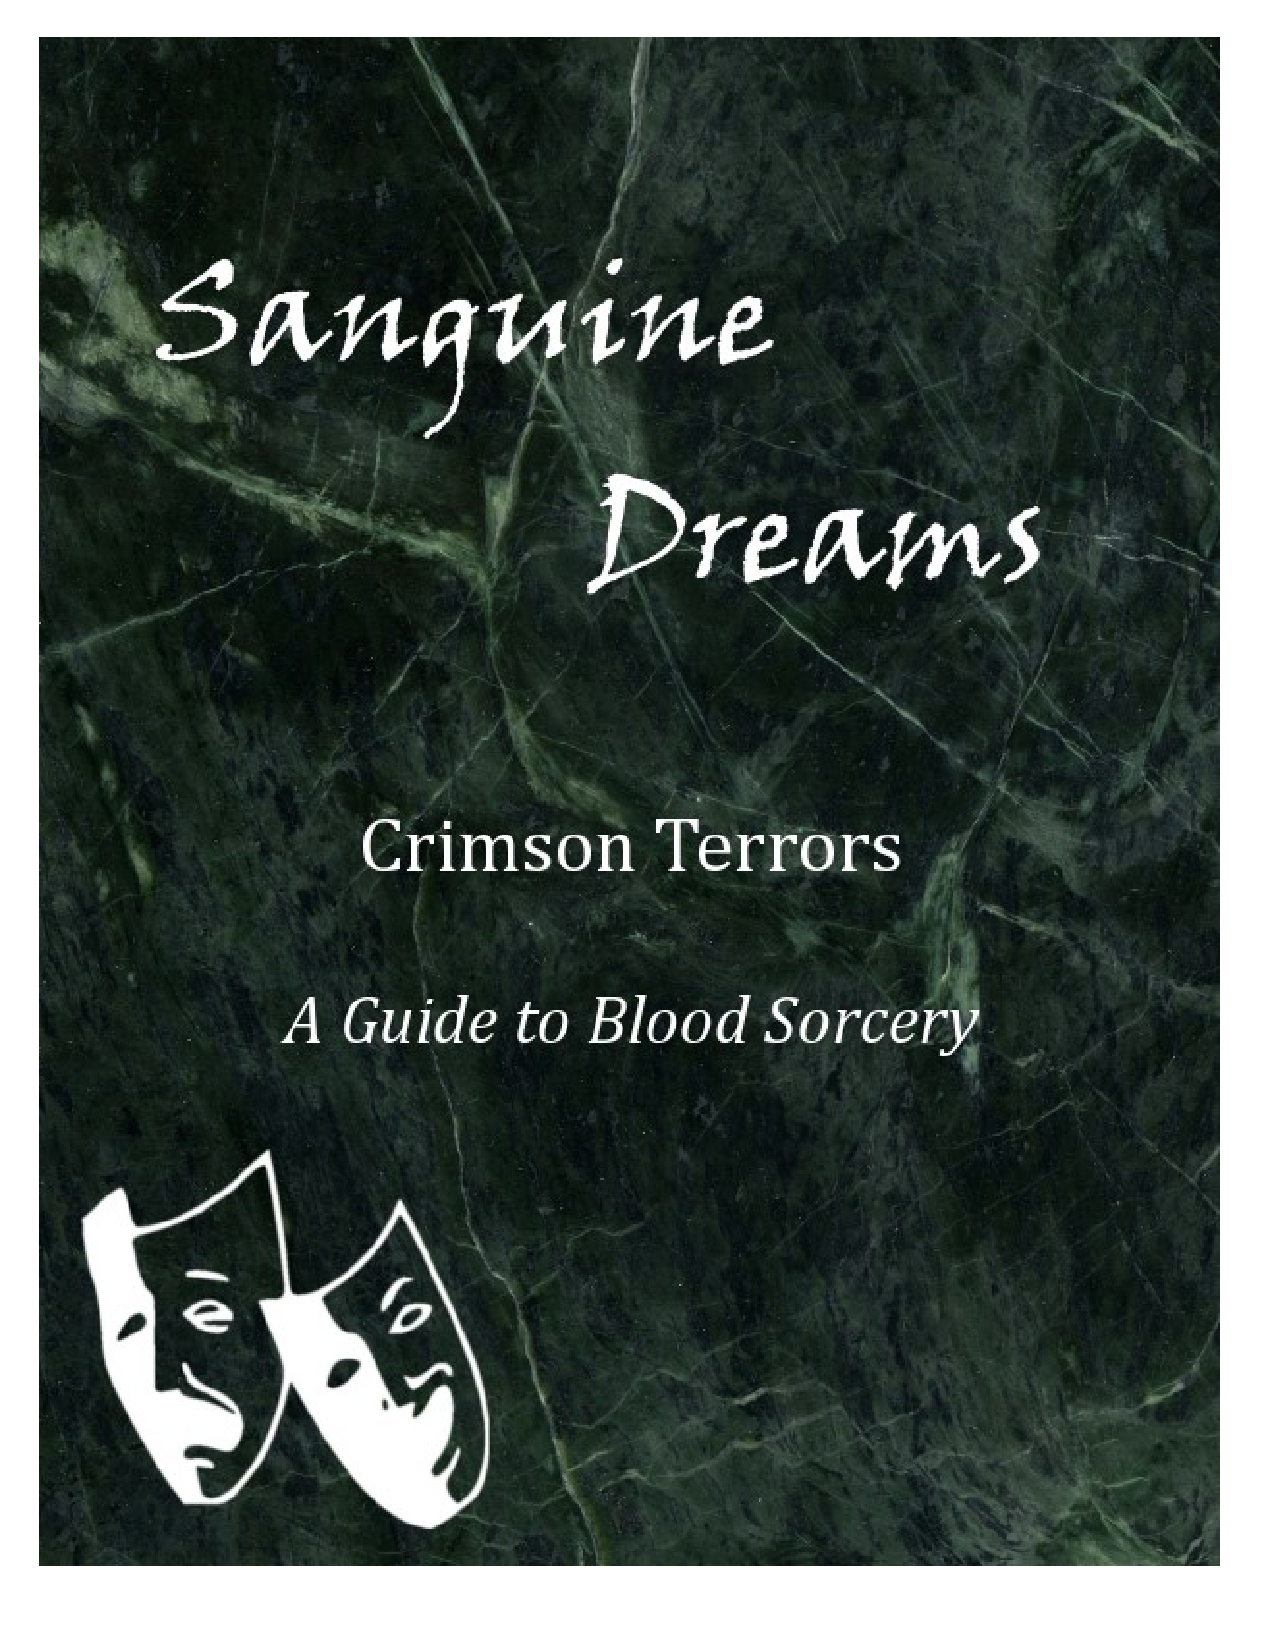
\includepdf{Crimson_Cover.pdf}
\ClearWallPaper					%% UNCOMMENT FOR PRINT VERSION %%%
\thispagestyle{empty}				%% UNCOMMENT FOR PRINT VERSION %%%
\mbox{}							%% UNCOMMENT FOR PRINT VERSION %%%
\newpage			

\addtolength{\wpXoffset}{-4pt}
\addtolength{\wpYoffset}{1pt}
\CenterWallPaper{.86}{background4.png}		% Uncomment if regular style
\begin{titlepage}
\thispagestyle{empty}

\begin{center}

\vspace*{5cm}

\textsc{\Huge Sanguine Dreams}\\[0.5cm]

\textsc{\LARGE 1990s \emph{Vampire: the Masquerade}}\\[0.5cm]

\TitleRule \\[0.6cm]
{ \LARGE Crimson Terrors}\\[0.2cm]
{ Blood Magic Supplement } \\[0.4cm]
{ Updated June, 2016 }\\[0.4cm]		% Revision Date
\TitleRule \\[1.5cm]

\textit{With special thanks to}\\
\vspace*{0.5cm}

\begin{minipage}{0.4\textwidth}
\begin{flushleft} \large
\textsc{Brandon Lake}\\
\textsc{Sarah Sudol}\\
\end{flushleft}
\end{minipage}
\begin{minipage}{0.4\textwidth}
\begin{flushright} \large
\textsc{Tony Valerro}\\
\textsc{and our players}\\
\end{flushright}
\end{minipage}

%\vspace{1.5cm}
%\emph{(( Release Candidate 2 ))}

\vspace{3.5cm}			% Add back in after the above is gone
%\vspace{2.0cm}
{\large https://sanguinerpg.com}

\end{center}
\end{titlepage}


		%
%Create the dedication page after the title
\newpage
\ClearWallPaper
\thispagestyle{empty}
\vspace*{6.0cm}
\begin{center}
	{\large {\color{gray}\emph{``There is always danger for those who are afraid.'' \\[1cm] \hspace{12ex} --- George Bernard Shaw}}}
\end{center}

% Table of Contents
\newpage
%\hfill \\[2cm]
\setcounter{tocdepth}{3}				% Set to 1 to only include Chapters
\setcounter{secnumdepth}{1}				% Removes numbering for subsubsections
\pagenumbering{roman}
\setcounter{page}{1}
\tableofcontents				%

\newpage						%%% UNCOMMENT FOR PRINT VERSION
\thispagestyle{empty}			%%% UNCOMMENT FOR PRINT VERSION

%	No intro page

 % All content
\mbox{}
\newpage						%
{\fontsize{8}{9}\selectfont				% Comment if full-page
\frenchspacing
\pagenumbering{arabic}
\pagestyle{fancy}
\setcounter{page}{1}
\CenterWallPaper{.85}{background5.png}		% Uncomment if not full-page
\addtocontents{toc}{\protect\setcounter{tocdepth}{2}}
\section{Introduction}
\label{sec:introduction}
In this supplemental rule guide for \emph{Sanguine Dreams}, the strange and wondrous Disciplines 
of Thaumaturgy and Necromancy are explored, along with the Clans who can wield 
those amazing powers.  These specific Disciplines have significant advantages over those which 
come naturally to other Clans, but also significant drawbacks both in the raw costs to cast 
the spells and the secrecy to which their practitioners must keep.

\textbf{This guide is not designed to be read by every player} -- the contents here are some of 
the most secret and carefully-guarded in all of kindred society, and are far from general knowledge.  
The Clans which wield these powers often have complex and complicated internal structures, invisible 
to those outside, and the Storytellers highly recommend players not actively role-playing 
characters in those Clans to skip this guide entirely.

Thaumaturgy and Necromancy differ from other Disciplines by encompassing a wide range of powers, 
divided into paths, as well as complicated rituals which can provide longer-lasting effects than 
most any other power in the game.  Practitioners of these dark arts are loath to divulge their 
secrets, even descriptions of what is or isn't possible, and those who talk too freely are often 
``called away'' unexpectedly, not to be seen by local kindred again.

This guide should be considered the authoritative source of all rules related to the use of these 
two Disciplines, though it makes frequent reference to other source material previously published 
by White Wolf, the original creators of \emph{Vampire: the Masquerade}.  If ever there is a 
conflict between the original books and this volume, the rules presented here and in other guides 
created for \emph{Sanguine Dreams} take presidence.

The powers of Thaumaturgy and Necromancy are wide and varied, and the Storytellers encourage 
players to remember the Golden Rules, to expand upon and elaborate on the thematic elements which 
make these Disciplines so interesting.  When in doubt, please see a Storyteller.

The contents of many sourcebooks went into the construction of this document, and where available 
each power's source has been included in its writeup.  Often the original source provides additional 
thematic elements or role-play opportunities with these powers, but the final mechanics that will 
be used in \emph{Sanguine Dreams} are all presented in this volume, disregarding the original 
writeups.  As a unilateral rule powers not appearing in this volume are not approved for play. \\

\begin{minipage}{0.5\textwidth}
   \begin{flushleft}
	{\scriptsize
	\emph{SD} --- Sanguine Dreams-specific \\
	\emph{LotN} --- Laws of the Night \\
	\emph{Grey} --- Laws of the Night (2\textsuperscript{nd} Ed) \\
	\emph{ST} --- Storyteller's Guide \\
	\emph{BM} --- Blood Magic (2\textsuperscript{nd} Edition) \\
	\emph{Elysium} --- Laws of Elysium (2\textsuperscript{nd} Ed) \\ }
	\end{flushleft}
\end{minipage}
\begin{minipage}{0.5\textwidth}
   \begin{flushleft}
	{\scriptsize 
	\emph{Clan} --- Clanbook \emph{(Clan)} \\
	\emph{Night} --- The Long Night (Dark Ages) \\
	\emph{Anarch} --- Guide to the Anarchs \\
	\emph{NYBN} --- New York by Night (2\textsuperscript{nd} Ed) \\
	\emph{CamTT} --- Guide to the Camarilla (Table-Top) \\
	\emph{BS} --- Blood Sacrifice (2\textsuperscript{nd} Ed) \\ }
	\end{flushleft}
\end{minipage}			% General overview and setting information
\section{Practitioners of Magic}
\label{sec:clans}
All throughout kindred history rumors have surfaced about strange abilities attributed 
to specific Clans, powers shrouded in mystery and unavailable to any other Blood.  The 
Clans who have managed to develop these impressive Disciplines are few and far between, 
and guard their secrets with the utmost ferocity, taking exacting and sometimes fatal 
vengeance against those who pry too deeply.

Across the whole of kindred kind there are only three Clans who can claim to have control 
over Thaumaturgy, and only one that can call themselves masters of Necromancy.  Rare 
cases of small or historic bloodlines being able to wield these powers have been known, 
but their numbers are so few or so far in the past as to put them out of the thoughts of 
all but the most meticulous of kindred scholars.

Each Clan's sourcebook has great information about the history, culture, and internal 
structure of the Clan and their outlook on kindred existence.  The information presented 
below is meant to be an overview or supplement to the works already published by 
White Wolf.

\subsection{Clan Tremere}
\label{sec:tremere}
The undisputed masters of Thaumaturgy, Clan Tremere claims that they alone developed 
the rites and rituals required to bend the very fabric of reality to their whims.  
Almost invisible to those outside the Clan, a rigid and well-established hierarchy 
controls almost all aspects of a Tremere's study of Thaumaturgy and interactions with 
others who share their blood.  Groups of Tremere are organized into Chantries, usually 
no more than one per metropolitan area.  A great deal of competition takes place 
between the members of a Chantry, each fighting for recognition and promotion within 
the Clan structure, called ``the Pyramid,'' but when faced with an external threat the 
Clan unites as one well-organized and unstoppable force.

\subsubsection{Organization}
At the lowest level, and most relevant to the characters of \emph{Sanguine Dreams}, are 
the \textbf{Apprentices}.  Each Chantry is made up of Apprentices, who are designated 
according to their ability and benefit to the Clan.  Ranked from the first to the seventh 
``Circle of Mystery,'' most player-characters will fall between the ranks of A3 and A6.  
Note that rank has very little to do with kindred age or experience, and just as at times 
characters will be elevated, so too may they be demoted if they earn their superiors' 
displeasure.  As an Apprentice moves up in Rank, they are given more responsibility but 
also greater access to powers and areas of study.

Apprentices of the First and Second Circles of Mystery are functionally under Accounting, 
unable to leave the Chantry or the presence of a higher-ranking Tremere for any reason.  
Once an initiate has demonstrated a proper command over Thaumaturgy and knowledge of 
kindred society are they raised to the Third Circle.

Apprentices of the Third, Fourth, and Fifth Circles serve as the backbone of Clan Tremere, 
with increasing responsibilities and research opportunities.  These kindred have proven a 
basic competency of Thaumaturgy and have shown their value to the Clan as a whole.  Very 
often the Primogen, as public face of the Clan, comes from these ranks as higher-level 
Apprentices are too busy to take on such outward-facing responsibility.

Apprentices of the Sixth and Seventh have proven themselves highly proficient not only in 
their mastery of Thaumaturgical power but also individual specializations therein, often 
fulfilling a specific niche unavailable to other kindred.  The highest-ranking Apprentice 
in a Chantry, almost always at this level, is called the ``High Apprentice'' and it is 
often their responsibility to oversee the education of less experienced magi, even if 
not directly.

Each Chantry is lead by a \textbf{Regent} who serves as master of the house.  Just as 
there is functionally no appeal if a kindred dislikes their Prince, there is almost no 
ability to go over a Regent's head when it comes to the conduct or management of a Chantry.  
These kindred, also ranked from the First to the Seventh Circles, have vast stores of both 
knowledge and power and have at least a base understanding of all aspects of Thaumaturgy, 
including the mastery of rituals required to create, maintain, and defend a Chantry.  Often 
a Regent's rank is directly related to the size or importance of the Chantry over which they 
are called to preside, but such is not a universal rule.

Each Regent reports to a \textbf{Lord} who oversees large geographical areas and the 
management of each chantry therein.  These beings are as far above Regents as Regents are to 
Apprentices, their power and understanding of the mystic arts almost unfathomable to younger 
kindred.  When a Regent issues a directive, it can be said to come from the Lord's will.  When 
a Lord issues a directive, it can be said to come from the very Clan itself.

There are higher levels of the Tremere hierarchy, but even the most effective Apprentice has 
scarce more than a whisper's chance of meeting someone in those lofty positions unless they 
have made a series of truly regrettable decisions.

The Clan has codified a strict hierarchy of which paths and rituals can be studied, depending 
an Apprentice's Circle of Mystery rank.  It is unlikely that most have even heard of powers 
more than two ranks above their own, but local conditions and needs sometimes force 
Regents to authorize otherwise undeserving kindred to learn the secrets of their betters.

\subsubsection{Common Powers}
Every Tremere begins their life as a student of \emph{Thaumaturgy} with the study of the \emph{Path of Blood}, 
from which the core of the Clan's power stems.  As they grow and advance many who are more 
combat-oriented learn \emph{Lure of Flames} or \emph{Movement of the Mind} while others 
take a more esoteric role, studying \emph{Spirit Manipulation} or \emph{Oneiromancy}.

Clan Tremere has the largest collection of paths and rituals available to them, and have the 
easiest time learning them of all the thaumaturgically-active Clans, its internal hierarchy notwithstanding.


\subsection{Clan Assamite}
\label{sec:assamite}
Description of Clan Assamite and its history (the curse, Alamut, taking contracts, et cetera)

\subsubsection{Organization}
Talk about the types of Assamites (particularly how we only allow the actual assassins as PCs, 
not Viziers or others) and their roles here

\subsubsection{Common Powers}
Discuss paths of Thaumaturgy "common" to select Assamites and what they do to share powers.  
Discuss the rituals available/limited to them.


\subsection{The Followers of Set}
\label{sec:settite}

\subsubsection{Organization}

\subsubsection{Common Powers}


\subsection{Clan Giovanni}
\label{sec:giovanni}

\subsubsection{Organization}

\subsubsection{Common Powers}
				% Clans
\section{General Rules of Blood Magic}
\label{sec:rules}
The powers of Thaumaturgy and Necromancy are wide and varied, with effects that have the capacity 
to alter the game or characters' interactions far more than any other Disciplines in the game.  
Rules specific to each power are presented in their own sections, but the following rules apply to 
every use of blood sorcery, whether it is a ritual or regular Discipline.

\begin{itemize}
	\item This volume contains every power available to player characters and most powers available to 
	non-player characters.  It is not possible within the scope of a chronicle to develop a new path 
	or ritual for either Thaumaturgy or Necromancy.
	\item Nearly all powers require a challenge to be thrown, usually retested with the \emph{Occult} 
	Ability.  Each such challenge should be thrown with a Storyteller present, due to the complexity 
	of interactions with other powers or characters.
	\item Unless otherwise specified, the casting of Thaumaturgy or Necromancy is an obvious and evident 
	process, requiring both hand gestures and vocal incantations.  If used in combat, the use of these 
	Disciplines takes the entire combat turn and can not be sped up with Celerity.  All Thaumaturgy and 
	Necromancy powers resolve at the end of the combat turn unless otherwise specified.  Even with 
	Celerity the casting character may not perform additional actions save for movement.
	\item Some powers allow for the creation or alteration of items.  No such item may have more than 
	one magical affect upon it at a time; at Storyteller discretion either the more powerful effect 
	takes precedence or the newest effect supplants the old.  This prohibition also applies to the 
	Quietus powers of \emph{Scorpion's Touch} and \emph{Baal's Caress}, among others.
	\item Many powers require a Mental versus Physical Challenge.  Typically these challenges require 
	the defender to bid a Dexterity trait to avoid the power's effects.  If a victory condition is solely 
	damage, Stamina may also be used.  In all cases Storytellers are the final arbiter of which traits may 
	be used in a given challenge.
	\item Ranged powers require a ``line of effect'' when determining valid targets for a Discipline.  
	For a ranged subject to be a viable target there must be no solid barrier between you and, depending on 
	Storyteller fiat, the path must be relatively clear of obstruction.  Even transparent materials such as 
	glass will block ranged Disciplines.
\end{itemize}			% General Blood Magic Rules
%%%%%%%%%%%%%%%%%%%%%%%%%%%%%%%%%%%%%%%%%%%%%%%%%%%%%%%%%%%%%%
\addtocontents{toc}{\protect\setcounter{tocdepth}{3}}
\section{Thaumaturgy}
\label{sec:thaumaturgy}
Placeholder text for the introduction to Thaumaturgy, if we need one
			% Thaumaturgy Intro
\subsection{Thaumaturgy Paths}
\label{sec:tpaths}
The Discipline of \emph{Thaumaturgy} is divided into many paths, each with a different 
focus or theme.  All uses of the Disciplines listed in this section require a Blood 
expenditure, as well as any other listed costs.

Each Thaumaturge has a Primary Path of study which is determined by their Clan, and represents an 
affinity or focus that Clan has for a particular set of powers.  While learning other paths is 
possible, and often encouraged, certain conditions must be met before Storytellers will approve 
the purchase of additional dots in additional paths.

Before learning either of the Basic levels of a Secondary Path, the magus must have at least an 
Intermediate level of understanding in their Primary.  Similarly before gaining the Intermediate 
powers of a Secondary Path, they must have mastered the Advanced power of their Primary.  A 
similar restriction follows all future paths under study, called ``Tertiary Paths,'' and which 
are limited by one's comprehension of their Secondary Path.  Once a character has mastered both 
their Primary and Secondary paths, there is no longer a restriction on what the character can 
learn, from a mechanical perspective.

Almost all users of Thaumaturgy however must ask permission from their superiors before embarking 
on new studies or advancing existing Paths.  This serves as a fantastic opportunity for role-play 
as the student pleads their case, also ensuring the player knows what their character will be 
learning before diving in blindly.  In all cases, requests to advance one's knowledge of 
Thaumaturgy requires specific Storyteller approval.

As with all other Disciplines levels one and two are considered Basic, levels three and four 
Intermediate, and the final dot is considered the Advanced level.

\subsubsection{Alchemy (Chrysopoeia)}
Overlooked by most twentieth century thaumaturges, elder Tremere still practice this Path as a 
reminder of the principles modern blood magic is based on.  Dealing with Hermetic ideals of reality, 
and less practical applications thereof, this path transmutes one substance into another, normally 
without changing the form or function of the raw materials at hand.  Anyone hoping to utilize this 
Path must possess either two levels of \emph{Science: Chemistry} or four \emph{Academics} and must 
be working in a controlled environment, much akin a modern-day laboratory or clean room.   Each 
application of \emph{Alchemy} takes one hour per level being used, and the caster must have exacting 
knowledge of the chemical makeup of the material they are working with.  All levels require a 
Static Mental Challenge to succeed, with a difficulty set by the Storyteller, retested with 
the appropriate \emph{Science}.  \emph{(Availability: A4.  Source: ST p.47)}

\begin{description}
	\item[1 -- Commuta:]  This power allows the thaumaturge to change the state of a single, uniform 
	material; solid to gas, gas to liquid, liquid to solid, or the reverse.
	\item[2 -- Conforma:]  With this power the caster can separate out simple elements, creating loose 
	clouds of hydrogen and oxygen from water, or forcing liquid into a specific, simple solid shape.
	\item[3 -- Scinde:]  At this level complex form changes can be made, such as changing water into 
	breathable oxygen and free hydrogen, compounds into piles of separate elements, and so forth.
	\item[4 -- Mutate:]  Minor shifts in composition are now possible, such as shifting a single element's 
	atomic number by up to five on the Periodic Table of Elements.
	\item[5 -- Transmutate:]  The thaumaturge may now force radical shifts in composition, functionally 
	allowing them to transform any starting element into any other element.  Any use of this power will 
	be carefully overseen by the Storytellers to ensure proper game balance.
\end{description}

\subsubsection{Biothaumaturgy (Bioconmutatus Arcanum)}
A truly macabre path which deals with flesh in all states, is possibly the inspiration for such works 
of fiction as ``Dr. Frankenstein,'' and those who practice it are regarded with curiosity and revulsion, 
even within the Sabbat which developed it.  This Path does not require any Blood traits to be spent in 
its use, but individual costs are listed under each power.  Anyone wishing to utilize this power must 
possess at least three levels of \emph{Science: Biology} (or similar) and one dot of \emph{Medicine}.  
All retests are performed with the relevant \emph{Science}, and uses of this power must be performed in 
a workshop or laboratory prepared for the purpose.  \emph{(Availability: Sabbat.  Source: ST p.48)}

\begin{description}
	\item[1 -- Thaumaturgical Forensics:]  After a week's worth of study on a plant, animal, or 
	supernatural tissue sample and succeeding on a Static Mental Challenge, difficulty set by the 
	Storytellers, this power allows for a wealth of information to be obtained, far beyond what 
	``normal'' forensics or genetic testing would yield.  The information will always be physical 
	in nature, and it is up to the Storyteller how much is gleaned under a given examination.  
	This study destroys the sample and requires the expenditure of one Willpower at the start of the 
	week.
	\item[2 -- Thaumaturgical Surgery:]  Further studies into this Path yield amazing recuperative 
	abilities for a caster's patients.  By spending up to three Mental traits and a like number of 
	Blood, neither of which can be replenished by any means until the next evening, the caster can 
	force a subject to heal.  For each Mental trait spent one wound of the caster's choice downgrades 
	from Aggravated to Lethal, or Lethal to Bashing, or Bashing to nothing, which requires ten minutes 
	of dedicated ``surgery'' time per wound.  This power may only be used once per evening, regardless 
	of the number of available patients.  The subject must spend the majority of the rest of the night 
	in the laboratory, under the caster's care, for this power's effects to hold.
	\item[3 -- Lesser Animation:]  Imbuing an intact, dead being with a part of their own undead life 
	essence, a biothaumaturge can create small golems, no larger than dogs, to fulfill simple 
	instructions.  These animated corpses have reduced Physical traits and wound levels from what they 
	had in life, and zero Mental or Social traits, though they are immune to \emph{Dominate} and 
	Social-based powers as a result.  Immediately crumbling to dust if exposed to sunlight or fire, 
	these creatures can nevertheless follow a single basic, one-sentence command issued by the caster, 
	which it will follow to the best of its ability for the rest of its pitiful life.  Animating a 
	corpse requires at least seven nights of preparation and experimentation, culminating in a 
	Static Mental Challenge with a difficulty set by the Storytellers.  The use of this power requires 
	the permanent sacrifice of a Blood trait which remains unavailable until the creature is destroyed.
	\item[4 -- Greater Animation:]  As \emph{Lesser Animation} save the caster may now reanimate 
	creatures of almost unlimited size, or graft additional body parts onto existing animated corpses.  
	To awaken larger creatures requires two weeks of study while making modifications requires only a 
	single week of experimentation.  In both cases the biothaumaturge must succeed in a Static Mental 
	Challenge, with a difficulty set by the Storyteller.  Truly large beings may require the sacrifice 
	of multiple Blood points.
	\item[5 -- Cognizant Construction:]  With three weeks of work, the caster may imbue their creation 
	with some semblance of mental acuity, though always less than it had in life, its intellect turned 
	to sinister purpose.  While it now loses its immunity to \emph{Dominate}, the caster may now change 
	the orders given to such a creation at any time, unlike with lesser beings.  All creatures so 
	created require a difficult Static Mental Challenge.
\end{description}

\subsubsection{The Path of Blood (Rego Vitae)}
The Primary Path for all Tremere characters, this path represents a near-total mastery of the 
vitae which fuels their night to night existence, both within themselves and, eventually, within 
others.  \emph{(Availability: any Tremere.  Source: LotN p.177)}

\begin{description}
	\item[1 -- A Taste for Blood:]  By imbibing a trace amount of another's vitae (which can form 
	or advance a Blood Bond), you may learn the following information about the individual:  
	how much Blood is currently in their system, how recently they have fed, if and to what degree 
	they are wounded, a vampire's Generation, and whether or not the vampire is a Diablerist.
	\item[2 -- Blood Rage:]  Requiring light contact, which may necessitate a Physical Challenge, this 
	power allows you to force another kindred or ghoul to spend a single Blood trait in any fashion 
	you desire, even over the limits of their Generational ability to do so in a single turn.  This 
	power is sometimes used to bring kindred out of torpor, forcing their bodies to heal.
	\item[3 -- Blood Potency:]  This amazing power allows the thaumaturge to temporarily lower their 
	Generation by spending two Mental Traits for each Generation, to a maximum of six Traits.  This 
	power lasts for a scene or hour and while so affected you may claim your temporary Generation for 
	the efficacy of Dominate, total blood pool, and trait maximums.  If you are diablerized or attempt 
	to sire childer while in this state however, use your actual Generation.
	\item[4 -- Theft of Vitae:]  By engaging in a Mental versus Physical Challenge with a target within 
	fifty feet, you are able to effectively feed at range.  This power requires the expenditure of up 
	to three Mental Traits before throwing the challenge, which determines how many Blood traits you 
	can steal from another, one per.  Blood gathered this way flies directly from your target into your 
	hands and is not purified in any way -- using this power on another vampire creates a Blood Bond, if 
	the blood is tainted you will become sick, et cetera.  This power is an enormous breach of the Masquerade.
	\item[5 -- Cauldron of Blood:]  After establishing a firm grip on a target, a thaumaturge can boil 
	the literal blood out of them.  By spending up to three Mental Traits and then engaging in a Mental 
	versus Physical Challenge (Stamina traits are a valid defense), you may cause a like number of Blood 
	traits to boil out of their body, causing one Aggravated wound apiece.  Mortals are almost instantly 
	killed by this attack and you may not successfully boil more Blood than they currently possess.
\end{description}

\subsubsection{Path of Curses (Crea Maledicta)}
Rumored to exist for as long as vampires have been studying blood sorcery, this Path provides powerful 
hexes and curses upon its victims.  While powerful this Path is also dangerous, for each incantation 
must be said directly to the target.  The thaumaturge wishing to use this power upon another must have 
a symbolic link to fuel the magic -- a bit of blood, a treasured object, or the like, and then best 
the target in a Social challenge, retested with \emph{Intimidation}.  A new symbolic link is required 
for each casting, even against the same target.  All powers last until sunrise unless otherwise specified, 
or until lifted by the caster, whichever is first.  \emph{(Availability: Non-Camarilla.  Source: ST p.56)}

\begin{description}
	\item[1 -- Stigma:]  This power marks the target with an aura of revulsion, making others uncomfortable 
	to be around them.  The subject of this curse must bid an extra trait in all Social challenges, and loses 
	all ties in such challenges.  This power lasts until the following sunset.
	\item[2 -- Malady:]  If successfully invoked this power afflicts the subject with a terrible sickness, 
	causing them to suffer a two trait penalty on all Physical challenges due to discomfort.  The illness 
	is much like the flu, with similar symptoms, which the victim should role-play appropriately.
	\item[3 -- Pariah:]  Twisting the perceptions of a victim's peers, this power forces all who look upon the 
	subject to see their most hated foe, though their voice is unaffected.  This power works as an offensive 
	\emph{Mask of a Thousand Faces}, save that the person under its effects cannot break it themselves.  \emph{Auspex} 
	can test to see through this power normally.
	\item[4 -- Corrupt Body:]  By denouncing the physical form of the accursed, the caster forces the victim's 
	body to warp into a grotesque parody of what it once was.  This outward caricaturing brings with it mind-wracking 
	pain, and subjects who have undergone this curse are often scarred both physically and mentally.  This power 
	reduces the target's maximum Physical traits to half, confers two Negative Physical traits chosen by the 
	Storyteller, and renders all Appearance-based Social traits unavailable for the duration of the curse.  The 
	target must also spend one full turn doing nothing but writhing in agony as the curse takes hold.
	\item[5 -- Fall from Grace:]  If successful in the application of this power, the thaumaturge lays a truly 
	disastrous curse upon the victim, ensuring the odds are always stacked against them.  The subject loses all 
	ties in all challenges and cannot use any retests, including those given by Merits or Disciplines.  Any use 
	of this power will be carefully overseen by the Storytellers to ensure proper game balance.
\end{description}

\subsubsection{The Path of Conjuring (Crea Materia)}
Creating objects from nothingness is the practice of Conjurers who draw on their own knowledge and experience 
to craft items and materials from empty space itself.  Objects created with this path are generic, without 
distinguishing marks or ornamentation, and are the same very time.  It is impossible for a caster to conjure 
anything larger or heavier than themselves, and they must have a working knowledge of the object to be brought 
forth, which may require specific Abilities.  Any object that is created with this power that is broken apart 
or otherwise severely damaged will melt into unusable sludge as the spell fades away.  All items created through 
this Path must be represented by item cards signed by a Storyteller which includes the amount of Mental Traits the 
caster had at the time of casting.  \emph{(Availability: Tremere A5.  Source: LotN p.182)}

\begin{description}
	\item[1 -- Summon the Simple Form:]  You are able to create basic objects made of only one material, little more 
	than chunks of matter.  Lacking any complex or moving parts, sample objects include a rod of metal, a club, 
	wooden stake, a rock, or lump of coal.  All objects created with this power require a Mental Trait to be 
	sacrificed at the start of each turn, or roughly three seconds, or the object dissolves.
	\item[2 -- Permanency:]  After an object is created with \emph{Summon the Simple Form}, spend three additional 
	Blood Traits to invest the creation with the gift of continued existence, no longer requiring additional upkeep.
	\item[3 -- Magic of the Smith:]  Objects that contain mixed materials, moving parts, and are complicated in 
	form or design are now within the conjurer's ability to create.  As long as they are familiar with an object's 
	workings, represented by dots in a relevant Ability, they can create a relatively plain copy of it out of thin 
	air.  Creating an object with this power costs five Blood traits instead of the usual one, and includes the 
	effects of \emph{Permanency} at no additional cost.
	\item[4 -- Reverse Conjuration:]  By spending a full turn in concentration a conjurer may unweave any item created 
	by this Path, banishing it wholly into the nothing from which it emerged.  A caster's own objects may be dismissed 
	without a challenge, but objects created by others requires a Static Mental Challenge versus the number of traits 
	listed on the item card.  Without the use of other powers there it is not usually possible to determine whether 
	an object is real or conjured.
	\item[5 -- Power Over Life:]  Though you cannot create true life, through this power you can create a creature that 
	has at least the semblance of it.  Using this power requires the expenditure of ten full Blood traits, and the creation 
	lasts for one week before dissolving.  These simulacra have no will of their own and follow your commands mindlessly, 
	doing their best to follow simple directions.  At all times the actions and statistics of a creature conjured with this 
	power are under the control of the Storytellers.
\end{description}

\subsubsection{The Focused Mind (Patet Mentis)}
A truly rare Path, students of its teachings require serenity and dedication to train in, aspects often lacking in the 
modern, chaotic nights.  Its powers provide a thaumaturge with powerful cognitive abilities, perhaps only recently 
paralleled with the rise of computers.  Any wishing to learn this Path must have at least seven permanent Mental traits.  
\emph{(Availability: A6.  Source: ST p.50)}

\begin{description}
	\item[1 -- Readiness:]  By succeeding a Static Mental Challenge against five traits the thaumaturge becomes more alert 
	and aware of their own memory.  For the next scene or hour the caster is up three traits Mental Challenges related to 
	leaps of logic, investigation, memory, or reasoning, at Storyteller discretion.
	\item[2 -- Centering:]  Speaking soothing words as a mantra, this power's effects may be used by the caster or upon 
	another willing subject.  By sacrificing up to three Mental traits and then succeeding on a Static Mental Challenge 
	against six traits, the subject is unaffected by wound penalties---Bruised, Wounded, or Incapacitated---and gains one 
	trait to resist persuasion per Mental trait sacrificed.  These bonus traits may be used in challenges to resist or 
	remain in frenzy, and challenges against mood-altering Disciplines.
	\item[3 -- One-Tracked Mind:]  Narrowing another's focus to a single desire, with a successful Contested Mental 
	Challenge and one full turn of conversation, the thaumaturge ensures that the subject will continue to fixate upon a 
	single thought or action that was undertaken immediately before or during the casting of this power.  This power lasts 
	a single scene or hour, until the individual is the subject of violence, or until their task is completed.  While so 
	affected this power's target receives a one trait bonus on all challenges related to their focused task.
	\item[4 -- Dual Thought:]  By spending a Willpower the caster may now take a Mental action during the Swiftness 
	combat round in the following combat turns, excluding other uses of \emph{Thaumaturgy}.  Once cast the thaumaturge 
	could \emph{Dominate} two different people per turn or work through logic problems with blinding speed.  This power 
	does not reduce or remove any cost associated with such actions, and lasts for either a single combat scene or ten minutes.  
	This power cannot be combined with \emph{Celerity} to receive two different actions in the Swiftness round.
	\item[5 -- Perfect Clarity:]  Steeling their resolve against all aggressions, the thaumaturge who has reached this level 
	of mental focus can shrug off external influences with a moment's concentration.  By spending a full turn in whispered 
	meditation and spending a Willpower, the caster becomes temporarily immune to all sources of frenzy, gains a 
	two-trait bonus to all defensive challenges, and all opponents attempting to influence or control the thaumaturge in any way, 
	including through \emph{Dominate} or \emph{Presence}, lose all ties to do so.  This power lasts for one combat scene 
	or ten minutes.
\end{description}

\subsubsection{Hands of Destruction (Perdo Materia)}
Magicians within the Sabbat have turned their focus toward violent and brutal applications of Thaumaturgy, and so have 
wrought this Path, which is rumored to have come from pacts with infernal demons.  As with all powers, effects which require 
touch first require a Contested Physical Challenge before the casting of the Discipline in question.  \emph{(Availability: 
Sabbat.  Source: LotN p.183)}

\begin{description}
	\item[1 -- Decay:]  Inanimate matter crumbles rapidly under your touch, aging a full year for each turn you 
	maintain contact, which can reduce wood or organic matter to rotted morass quickly, and even weaken metal or plastic 
	with sufficient time.  Undead flesh is susceptible to use of this power, though it only discolors and provides no 
	pentalties to the victim.
	\item[2 -- Gnarl Wood:]  Up to fifty pounds of wood, whether a door or a pile of split lumber, can be forced 
	to swell, contract, or twist into strange shapes with a glance.  Affecting wood held by someone, such a stake, requires 
	a Mental versus Physical Challenge.
	\item[3 -- Acidic Touch:]  Able to turn your own blood into a viscous and caustic acid, with a single touch you 
	can mar or burn most surfaces with a touch.  You may excrete the black ooze from any flesh on your body, which 
	does not harm you but deals a single Aggravated wound to any person or surface it touches.  This power may take 
	multiple applications to burn through solid, large, or particularly dense objects, at Storyteller discretion, and 
	cannot be flung or spit as a ranged attack.
	\item[4 -- Atrophy:]  With a single touch you are able to wither the limbs of your opponents, turning them into 
	useless, fragile appendages.  A limb struck in such a way shrivels, granting the victim \emph{Clumsy} and 
	\emph{Lame}, which can be stacked up to four times, once each per limb successfully struck.  A victim without 
	arms cannot grapple or wield weapons, a victim without functional legs cannot move.  While this effect is permanent 
	on mortals, vampires can heal the effects as if they were a single Aggravated wound per limb.
	\item[5 -- Turn to Dust:]  After maintaining a firm grip on your victim, engage them in a Mental versus Physical 
	Challenge.  Each Mental trait you expend before this challenge will age the target ten years if successful, causing 
	aged mortals to crumble into dust and vampires to become \emph{Repugnant} for the rest of the night.  This power 
	is only effective against living or undead targets; \emph{Decay} is for inanimate subjects.
\end{description}

\subsubsection{Hearth Path (Arcem Praesidio)}
Originally a collection of rituals, this Path deals with the security of one's haven.  All uses of this power 
may be ended at any time.  This Path only functions on locations important to the caster.  All powers last 
until the next sunset after casting.  \emph{(Availability: ???.  Source: ST p.51)}

\begin{description}
	\item[1 -- Guest's Herald:]  By placing small blood sigils on the inside of a door or other entryway, this 
	power creates a small auditory or visual effect that will alert the thaumaturge that someone has breached 
	the opening.  The signal can be anything the caster desires, so long as the effect is subtle.  The caster 
	must be within the haven for this power to have any effect.
	\item[2 -- Master's Order:]  Reaching a new level of connectedness with one's haven, through the use of this 
	power a thaumaturge instantly knows where each one of their inanimate possessions are within their haven, so 
	long as caster is inside.
	\item[3 -- Rhyme of Discord:]  This power befuddles the minds of intruders, causing them to become lost, 
	no matter how small or plain the haven actually is.  Any intruders must succeed in a Mental Challenge against 
	the caster, retested with \emph{Occult}, or else be trapped inside the haven until the thaumaturge breaks 
	the spell or it wears off naturally.  All individuals so affected will be unable to remember the details of 
	the protected haven even after they have left, unless at a future point they return when the haven is not 
	protected by this power.  All intruders may still fight and defend themselves normally, even if they could 
	not effectively pursue the thaumaturge.  This power does not require the thaumaturge to be home.
	\item[4 -- Temportal:]  A master of his haven, the caster may cause doorways inside to connect however he 
	chooses to link them, such as making shortcuts between floors or to a secured basement.  Anyone other than the 
	caster using or passing through the doors is unaffected by this power, often leading to a great deal of 
	confusion as the caster seems to disappear into thin air.
	\item[5 -- The Caultron's Rede:]  By imparting a small amount of awareness into the haven itself, a 
	master of the Hearth Path can ask any or all of the household items, or the building itself, what transpired in 
	or near the haven during the time this power was active, though it will not remember anything from previous 
	castings.  In cases of extreme danger, such as fire or an impending ambush, the voices of the haven will 
	actively scream out to the kindred, regardless of location.
\end{description}

\subsubsection{The Lure of Flames (Creo Ignem)}
One of the most feared powers in Thaumaturgy, this path allows the caster to control fire, that eternal 
enemy of kindred.  A practitioner of this path does not risk R\"{o}tschreck while in control of the flames, 
but secondary or unintentional fires pose a danger as normal.  The first three levels of this Discipline 
only require a single action of casting, not a full combat turn.  \emph{(Availability: any Tremere.  Source: 
LotN p.178)}

\begin{description}
	\item[1 -- Hand of Flame:]  Wreathe one or both hands in a flickering firelight, sufficient to light 
	a small room and cause other kindred to recoil.  This power lasts one scene or hour, or until you 
	decide to extinguish the flames.  All successful \emph{Brawl} attacks deal a single Aggravated wound, which 
	can be combined with powers such as \emph{Celerity} or \emph{Potence}.
	\item[2 -- Flame Bolt:]  By pointing at your target you may manifest a streak of flame which flies toward 
	your target.  With a successful Mental versus Physical Challenge you cause one level of Aggravated damage 
	to a victim within fifty feet.  If striking a readily flammable object such as a stack of papers, a 
	secondary fire may start.
	\item[3 -- Wall of Fire:]  Causing a column of flame to erupt from the ground, you can extend the fire to a 
	roaring curtain of flame.  The fire you cause reaches six feet high and can either form a straight line 
	barrier of ten feet or a circle with a six foot diameter.  If you attempt to conjure the wall beneath someone, 
	engage them in a Mental versus Physical Challenge.  If you win they take a single Aggravated wound as flames 
	erupt around them.  Anyone attempting to pass through or standing inside the barrier once created suffers a 
	level of Aggravated damage per turn.  The wall lasts for one scene or hour, or until you are knocked 
	unconscious, move fifty feet away, or dismiss it.
	\item[4 -- Engulf:]  By concentrating on a subject for a full combat turn you may cause them to burst into 
	flames, remaining alight until they are put out.  By succeeding in a Mental versus Physical Challenge the 
	victim suffers two Aggravated wounds as they are engulfed, perhaps causing other secondary fires to start.  
	At the end of each successive turn they suffer an additional Aggravated wound until they or a friendly 
	onlooker take a full combat turn to put themselves out.  Using this power on someone multiple times does 
	not increase the end of round damage, but does cause the initial wounds as normal.
	\item[5 -- Firestorm:]  Creating a swirling vortex of flames, any area you can see within fifty feet can 
	become the epicenter of a truly terrifying blaze.  Everything within a twenty foot diameter is subject to 
	roaring sheets of flame, which continue to strike until you dismiss them, move farther than fifty feet away, 
	or are knocked unconscious.  Make a mass Mental versus Physical Challenge with all in the area of effect -- 
	any who fail are struck in the initial blaze, suffering one Aggravated wound.  Everyone still inside the 
	area of effect at the end of successive combat turns suffer an additional Aggravated wound each turn.
\end{description}

\subsubsection{Mastery of the Mortal Shell (Dominum Pupa)}
This Path provides control over the physical workings of a body.  While devastatingly effective against living 
creatures, the undead are able to shrug off its influence by spending a Willpower at any time. This power 
cannot be used to re-animated corposes.   Unless otherwise stated effects last for a number of combat turns equal 
to the number of Mental traits spent in the casting, to a maximum of 3, and each power requires two challenges:  
one to establish a Physical touch, and a Mental versus Physical challenge to enact the power.  As normal these 
two challenges may be performed in the same action.  \emph{(Availability: A5.  Source: ST p.53)}

\begin{description}
	\item[1 -- Vertigo:]  After successfully touching a victim and besting them in a Mental challenge, the caster 
	can force their subject to suffer a wave of dizziness and disorientation, resulting in a one trait penalty to 
	all Challenges for the remainder of the scene, and may cause some effects such as acrophobia at Storyteller 
	discretion.
	\item[2 -- Contortion:]  With a successful touch to an arm or leg and follow-up Mental challenge, this power 
	forces the target to lose control of the affected limb, suffering the Negative Trait \emph{Lame}, and other 
	related penalties as determined by a Storyteller.  Additionally the caster may cast this upon themselves to 
	tighten their muscles, granting themselves two bonus traits for use when maintaining a grapple.
	\item[3 -- Seizure:]  Causing uncontrollable convulsions on their targets, this power forces the victim to 
	writhe on the ground, suffering one level of Bashing damage per turn, and making it impossible for them to 
	initiate Physical challenges, able only to defend with Stamina traits when applicable.  This power requires 
	the full concentration of the caster.
	\item[4 -- Body Failure:]  This power will all but instantly kill mortals as their autonomic nervous system 
	simply shuts down, and is extremely uncomfortable and painful to kindred.  By spending a Willpower the 
	caster causes the victim to suffer total system shock, causing three Lethal damage immediately and one more 
	each additional turn they are affected by this power, to a maximum of three.  Kindred affected drop to the 
	floor and may not initiate Physical challenges, only defending with Stamina traits where applicable.  Kindred 
	may overcome the effects of this power for one turn by spending a Willpower.
	\item[5 -- Marionette:]  After a successful Physical challenge to establish a grip, at any point later in the 
	same scene the thaumaturge may engage the victim in a Mental versus Physical challenge to establish dominance 
	over their entire body, forcing them to perform any physical actions desired, including speech.  The subject's 
	movements are not jerky or suspicious, acting naturally and ably as the body under control.  Because of the 
	intense concentration required for the use of this power, the thaumaturge cannot initiate challenges while 
	controlling a victim in this way.  The victim knows full well that their body has been usurped by an outside 
	force, but can do nothing to prevent acting in a way the caster desires for the duration.
\end{description}

\subsubsection{Movement of the Mind (Rego Motus)}
Through this power objects and even people can be manipulated from afar, though this control does not provide 
any tactile response.  Any subject within visual range can be a target for this power.  \emph{(Availability: any 
Tremere.  Source: LotN p.180)}

\begin{description}
	\item[1 -- Force Bolt:]  By winning a Mental versus Physical Challenge with your target you may knock them 
	off their feet until they spend one action to get up, or knock an item out of their hands.  This power can 
	also be used against unattended objects weighing less than one-hundred pounds, which may get shoved several 
	feet at Storyteller discretion.  This power requires only one action to use.
	\item[2 -- Manipulate:]  Through force of will you can exert fine manipulation over something at range.  
	With this power you may attempt to use any object you could normally wield with one hand, such as picking 
	something up, pushing a button, or firing a gun.  Using an object remotely requires your full concentration 
	and the difficulty of doing so requires that you bid an additional trait in all challenges related to the 
	item.  Control over the object continues so long as you maintain your concentration.
	\item[3 -- Flight:]  With this power you are able to lift a whole person, bodily lifting them from the ground.  
	Other large objects are also able to be lifted, but without fine control.  When invoking \emph{Flight} you are 
	able to lift any object of up to three-hundred pounds at a brisk walking speed (2 steps per combat turn).  
	This power lasts for as long as you are able to fully concentrate and see the target.  Lifting an unwilling 
	individual requires the success of a Mental versus Physical Challenge.
	\item[4 -- Repulse:]  Through the use of this power a physical shockwave blasts into your surroundings, knocking 
	objects and even people away from you.  You can affect any number of objects within your line of sight, and such 
	items fly up to twenty feet away.  Targeting individuals require a Mental versus Physical Challenge.  To strike 
	someone with a \emph{Repulsed} object requires a similar challenge, and likely deals one Lethal damage, at 
	Storyteller discretion.
	\item[5 -- Control:]  Proving mastery over telekineses, this power allows you to completely direct an object's 
	movements through the air, obeying your magical phrases and gestures.  Anything up to one ton in weight can be 
	the target of this Discipline, and you are able to manipulate it with the same dexterity as if you were using 
	both hands.  With this power you can use the item as a weapon, with damage depending on the object wielded, or 
	even control a melee weapon remotely, though this latter action requires you to bid two extra Traits for any 
	associated challenges.  People grabbed with \emph{Control} can be rendered nearly paralyzed or can be flung about 
	at your whim.  Initiating this power requires a Mental versus Physical Challenge, repeated every time you wish 
	to move the victim.  Exercising this level of manipulation requires your total concentration, and the power ends 
	if you become distracted, take another action, or lose sight of the subject.
\end{description}

\subsubsection{Neptune's Might (Rego Aquam)}
Though vampires often find swimming difficult, the sea has been a place of wonder and power for civilizations 
across the ages, and kindred kind is no different.  Once a thaumaturge reaches the Intermediate level of this 
path they may choose to specialize in either salt or fresh water, if desired.  This choice, or lack thereof, 
cannot be later unmade or changed.  If made, the caster receives a +2 bonus to using this power on the water 
they chose, but must bid two additional traits to affect the type of water they did not.  Blood is considered 
to be neither salty nor fresh for this purpose, and difficulties to manipulate it are unaffected.  
\emph{(Availability:  Tremere A4.  Source:  Camarilla Guide, p.81)}

\begin{description}
	\item[1 -- Eyes of the Sea:]  The thaumaturge may look deep into a body of water and see events that have 
	transpired in or around it, from the water's perspective.  Through this power the caster may see up to 
	twenty-four hours in the past.  By passing successive Simple Tests additional time may be observed as shown 
	below, though spending a Willpower counts as an automatic success.  This power can only be used on standing 
	water; lakes and puddles will do while oceans and rivers or wineglasses will not.
\end{description}

\begin{center}
\begin{tabular}{ | l l |}
	\hline
	\multicolumn{2}{| c |}{\textbf{Eyes of the Sea}} \\
	\hline
	1 Test & One additional week \\
	2 Test & One full month \\
	3 Test & One full year \\
	4 Test & Ten full years \\
	\hline
\end{tabular}
\end{center}

\begin{description}
	\item[2 -- Prison of Water:]  Exerting control over a body of water, you can force it to engulf and imprison 
	a victim.  A significant amount of liquid is required, though even a few gallons are enough to form binding 
	chains.  If insufficient water is present you must bid two additional traits in the initial Mental versus 
	Physical challenge to snare your target.  Mortals who are subject to this power may drown if you are not careful.  
	Spend additional Blood traits into creating this effect -- for every one you spend the prison gains two Physical traits.  
	Your level of \emph{Occult} is added as bonus Traits for any challenge the prison makes.  To break free, the 
	subject must defeat the prison in a Physical Challenge.  If desired you can order the prison to crush the 
	victim once per turn, initiating a Physical Challenge between the prison's traits and the subject's (Stamina 
	only, retested with \emph{Survival}).  Each successful challenge deals one Lethal wound.  The prison lasts 
	for one scene or hour, or until you move away from the area.  You must maintain line of sight to both the 
	prison and the source of water for the power to remain.
	\item[3 -- Blood to Water:]  Often used as a devastating assault against kindred and mortals alike, this power 
	allows the thaumaturge to transmute other liquids into water, even liquids inside a living body.  After establishing 
	a grip on the victim, requiring a Physical challenge, sacrifice up to three Mental traits and make a Mental versus 
	Physical challenge against the target.  If you succeed that many Blood traits are replaced with water, causing 
	excruciating pain and often death in mortals.  Vampires affected by this power have their current Blood pool reduced 
	and suffer penalties as if they had taken that many wounds, which automatically at a rate of one per hour and cannot 
	be healed by spending Blood.  Those possessing \emph{Fortitude} do not suffer the additional penalties, but still 
	lose vitae.
	\item[4 -- Flowing Wall:]  Commanding a powerful flowing wall of water to emerge from a sufficiently-sized body of 
	standing water is now merely a matter of effort for you.  Touch the surface of the water and spend two Willpower 
	traits.  For each Mental trait you then sacrifice you cause ten feet of watery barrier to appear in a single dimension, 
	either width or height, no more than one foot in thickness.  The wall can be placed anywhere in your line of sight and must 
	be formed in a straight line.  It remains in place until sunrise and cannot be climbed, though those attempting to pass 
	through it must make three Static Physical Challenges against your full permanent Mental traits (retested with 
	\emph{Athletics}).  Unless they succeed on all three Challenges they cannot pass.  This barrier also prevents travel by 
	psychic or spirit beings, who use their Mental traits instead (retest with \emph{Occult}).
	\item[5 -- Dehydrate:]  This level of mastery allows a thaumaturge to directly attack both mortal and supernatural 
	targets by stripping the water from their bodies at range.  Victims who die from this assault leave behind mummified 
	corpses.  Make a Mental versus Physical Challenge against a target within fifty feet.  If successful you inflict three 
	Lethal damage (if mortal) or strip three Blood traits (if kindred).  If a kindred is out of Blood they will suffer wounds 
	as if they were mortal.  Victim suffering damage must make a \emph{Courage} test against the amount of health levels 
	lost times two or collapse, overcome with agony for one turn.  Additionally this power may be used to dry wet clothing 
	or evaporate puddles.  
\end{description}


\subsubsection{Oneiromancy (Oneiromance)}
The unconscious thoughts and visions which swim through the slumbering mortal, and often immortal, mind have long 
been an interest to those wishing to gain a glimpse of the future that is to come, true diviners and paranoid 
Tremere alike.  Any use of this Discipline requires at least five minutes' worth of a dream-like trance during 
which time the practitioner interacts with the slumbering world.  \emph{(Availability:  Tremere A4.  Source:  ST's 
Guide, p.54)}

\begin{description}
	\item[1 -- Portents:]  By piecing together fragments of her own dreams, the magus may perform a reading of their 
	immediate future.  Casting this spell immediately after waking from a ten-minute dream trance and winning a 
	Static Mental Challenge against six traits provides for symbols and allegories directly related to an upcoming 
	event.  Multiple uses of this power will show the same vision until a new event becomes more pressing.
	\item[2 -- Foresee:]  This power allows the oneiromancer to use \emph{Portents} upon another sleeping individual, 
	so long as they are in the person's presence.  This power requires the caster to spend a Willpower if used on 
	a kindred.
	\item[3 -- Dreamspeak:]  At this level the thaumaturge may send messages, warnings, or even threats to a target 
	through dreams.  This power may be used upon anyone the magus has met, though the target must be asleep at the time 
	of casting.  Scenes lasting no longer than five minutes will repeat themselves through the victim's dreams, creating 
	a clear picture of the message upon waking.
	\item[4 -- Augury:]  Diving deeper into the collective unconscious, by spending half an hour in the dream trance and 
	winning a Static Mental Challenge against nine traits, the caster may receive a much clearer and deeper set of imagery 
	than what is found from \emph{Portents}.  The onieromancer may also use this power on anyone who has been the target 
	of a successful \emph{Foresee} or \emph{Dreamspeak} in the currentstory.  Remember that no matter the clarity, divination 
	is an imprecise and sometimes error-prone art.
	\item[5 -- Reveal the Heart's Dreams:]  By observing those around her, the thaumaturge gains incredible insight into 
	a subject's innermost fears and desires.  After spending at least five minutes in the company of the victim and winning 
	a Contested Mental Challenge (defended against with \emph{Subterfuge}), the caster may enter the dream trance later that 
	evening for fifteen minutes and receives the truth about either the subject's deepest fear or heart's greatest desire.  
	The answer to the question should be a driving force for the subject, not a passing interest or fear.  To use this power 
	on a mortal requires the expenditure of one Willpower at the time of the Challenge.  To use this power on a kindred 
	requires the expenditure of two Willpower.
\end{description}

\subsubsection{Path of Transmutation (Iter Transmutationibus)}
Regarded by elder Tremere as a poor man's \emph{Alchemy}, this path addresses the physical properties of matter within 
the thaumaturge's direct line of sight.  Its powers are very versitile, but can bring great destruction if used 
improperly.  All powers last for one scene or hour, or until dispelled by the caster.  \emph{(Availability:  Tremere A5.  
Source:  ST's Guide, p.60)}

\begin{description}
	\item[1 -- Fortify the Solid Form:]  By strengthening the bonds inside an object, the transmuter temporarily hardens 
	an object against damage.  An item with the Negative trait \emph{Fragile} loses it for the duration, armour becomes 
	more durable and able to soak an additional health level, and other uses have been employed by creative thaumaturges.  
	Enacting this power costs a Mental trait.
	\item[2 -- Crystalize the Liquid Form:]  This power will transform up to two pints of liquid into solid form, without 
	changing the substance's temperature or other physical properties such as its acidity or weight.  The solid form is 
	\emph{Fragile} and prone to breaking if not handled delicately, and all such transformed matter reverts to its natural 
	state at the end of the scene or hour.  This power costs a Mental trait, and only liquid that is open to the air can be 
	transmuted.  This power does not affect creatures who are already in a liquid form.
	\item[3 -- Liquefy the Solid Form:]  The reverse of the previous power, the thaumaturge must spend a number of Mental 
	traits relevant to the size of the object affected -- a hand-held object costs one, a door five, a barn eight or more.  
	At the end of the scene the puddle will revert to its natural form unless it is scattered.  This power does not work on 
	living or unliving beings.  Enacting this power requires a Static Mental Challenge against the number of traits 
	sacrificed.  Targets which may be affected by this power, such as by the floor becoming liquid, may receive a Dexterity-based 
	Challenge to jump away, at Storyteller discretion.
	\item[4 -- Goal:]  This power gives the transmuter control over the very air, solidifying it into an opaque, 
	indestructible and immobile barrier, even to kindred with \emph{Potence}.  \emph{Goal} has two different uses 
	which adds to its versatility:  an object or person may be encased in matter, or a wall created that is all but 
	impassible.  If creating a wall the caster must sacrifice a number of Mental traits relevant to the size of the wall, 
	as above.  If encasing a living being the caster sacrifices a like number of traits, usually five for a human-sized 
	creature, and engages in a Mental versus Physical Challenge, with the defender usually bidding a Dexterity-based trait.  
	The solid air is technically breathable, but mortals take a level of Lethal damage after being released as they cough 
	up the harsh material.  Creating a wall with this power requires a Static Mental Challenge against the number of traits 
	sacrificed.
	\item[5 -- Ghost Wall:]  At this level, thaumaturges find that even solid objects offer no resistance.  With 
	a full turn of concentration any inert material is rendered vaporous and may be passed through easily.  Floors underneath 
	foes may suddenly disappear, parachutes suddenly cease to work, and individuals can even suddenly find themselves falling 
	out of a speeding car that no longer supports their weight.  The caster spends a number of Mental traits relevant to 
	the size of the object being made gaseous, which returns to its former location after the power concludes.  Anyone standing 
	within the area of a recombining object suffers Aggravated damage, at Storyteller discretion.  Casting this level requires 
	a Static Mental Challenge against the number of traits sacrificed.  Any use of this power will be carefully overseen by the 
	Storytellers to ensure proper game balance.
\end{description}

\subsubsection{Vine of Dionysus (Dionysius de Vitis)}
Almost more a religion than a true thaumaturgical study, practitioners of this art are looked down upon by other 
Tremere for their lavish and hedonistic revelries.  Upon learning the first dot of this Path the thaumaturge automatically 
loses one permanent Willpower as they become ``addicted'' in its practices.  \emph{(Availability:  A5.  Source:  ST's Guide, p.61)}

\begin{description}
	\item[1 -- Methyskein:]  By making physical contact with their target and besting them in a Contested Mental Challenge, 
	the caster can make them feel drunk, suffering a one-trait penalty on all Dexterity- or Intelligence-related challenges, 
	forcing them to behave with the slurred speech and clouded judgment of intoxication.  If used on a mortal or ghoul three 
	nights in a row they can become addicted to this euphoria and may suffer ill effects per the \emph{Addiction} Flaw.
	\item[2 -- Omophagy:]  This power overwhelms the target with feelings of insatiable hunger, requiring only eye contact 
	and a Contested Mental Challenge to enact.  Mortals eat until they become sick and even then continue to want more, gorging 
	further after they vomit.  Kindred affected will not only drain a vessel completely of blood, but can sometimes even cause 
	them to feed upon other kindred, and even attempt to devour the victim's flesh, though without the merit \emph{Eat Food} this 
	behavior leads to predictably messy results.  A vampire affected by this power seeks out the easiest prey readily available, 
	at Storyteller discretion, and all victims lose awareness of their surroundings, in some cases causing likely breaches to the 
	Masquerade.  In no case will this power force a kindred to commit diablerie.  By spending a Willpower a victim can resist 
	falling to their urges for a few minutes, hopefully enough to exit the scene.  This effect lasts one scene or hour on vampires 
	and for the rest of the night on mortals.
	\item[3 -- Hamartia:]  With physical contact and a successful Contested Mental Challenge, the thaumaturge induces a severe 
	intoxication in the victim, to the point of perversity, delirium, and possibly torpid stupor.  A victim becomes two traits down 
	on all challenges for the remainder of the scene, and acts in a manner according to their Negative Traits and Flaws, and otherwise 
	as determined by the Storyteller.  If this power is used upon another practitioner of this Path however, in addition to the 
	penalties listed above they also gain a two trait bonus on all challenges of Strength.
	\item[4 -- Enthousiasm\'{o}s:]  Exuding powerful pheromones, the caster may make a Contested Mental Challenge with all 
	targets inside a ten foot radius.  Any victim of this power falls into a narcotic stupor as pleasant, dreamlike images dance 
	in their minds, causing them to giggle, dance, or just sit and sigh happily.  Targets under this power's effects gain 
	\emph{Submissive x2}, \emph{Lethargic}, and \emph{Witless} as Negative Traits for the remainder of the scene.  Kindred may 
	ward off these effects for one turn by spending a Willpower.
	\item[5 -- Oinos Aimatos:]  By invoking the essence of the wine god into themselves, the caster transforms his blood into a 
	powerful narcotic elixir.  For one scene, anyone imbibing even the tiniest drop of the thaumaturge's blood will be affected 
	as per \emph{Enthousiasm\'{o}s}.  This power costs an additional Blood and one Willpower to cast.  If Blood is placed into a 
	communal punchbowl or the like, its presence can only be detected by \emph{Heightened Senses} or other similar powers.
\end{description}
\subsection{Thaumaturgical Rituals}
\label{sec:trituals}

\emph{((General text about what rituals are and how they differ from paths here))}

\subsubsection{General Rules}
\begin{itemize}
	\item Learning a new ritual requires explicit Storyteller permission and role-play 
	justification for your character having learned it.
	\item All ritual effects cease at dawn unless otherwise specified, or upon the death of 
	all contributors to its casting.
	\item Rituals are listed with the Tremere Rank required to petition for its study.  Those 
	marked ``Any'' are available to all Tremere.  For other Clans, see availability writeups 
	in Section~\ref{sec:clans}.
	\item Most rituals do not cost Blood to cast, but do take a length of time specified either 
	by their level or individual description.
	\item All rituals require material components, many of which will be destroyed in the 
	casting.  The acquisition of these sometimes rare materials is an important aspect to 
	playing a Thaumaturge, and some may be very difficult to obtain.  Scenes to acquire 
	these resources should be run with the Storytellers.
	\item Rarely is a ritual's success or failure evident at the time of casting.
	\item Any items or locations enchanted with rituals must be represented by Storyteller-signed 
	item cards.
	\item Bonus traits and retests gained through rituals do not stack with those from Merits or 
	Ability Specializations, and must be similarly declared before a challenge is thrown.
	\item Rituals specifically noted as ``non-Camarilla'' or with a Clan name are only available 
	to characters that meet those requirements.
	\item Some rituals permanently reduce a character's available blood pool until ended.  Any 
	such reductions should be represented by an ``X'' through the character's final available blood 
	pool dot.  These powers lower a character's ability to store blood and as such the missing point 
	can not be filled.
	\item Some rituals can be ended at the will of the caster.  If in combat, the power ceases at the 
	end of the current combat turn.
	\item Each caster receives a free ritual when they increase their knowledge of their primary 
	Thaumaturgical path. This ritual can be at or below the new dot's level (Basic, Intermediate, Advanced).
\end{itemize}

\subsubsection{Basic Rituals}
All Basic rituals have a static difficulty of 5 traits and a casting time of 10 minutes unless otherwise stated.  
A character wishing to learn a Basic ritual must first have at least one dot of \emph{Thaumaturgy}. \\

\begin{description}
	\item[Bind the Accusing Tongue] \emph{(CamTT 109, A5)} \hfill \\ 
	This power lays a compulsion upon the target that prevents them from speaking ill of the caster, no matter the 
	consequences or circumstances.  Requiring an effigy of the target made with a lock of their hair and a black 
	silken cord, if successful this ritual requires the subject to beat the thaumaturge in a Contested Mental 
	challenge (both sides may retest with Willpower only) in order to speak ill of them for the remainder of the 
	scene.  The caster must have the effigy on their person and if the black cord is untied the ritual ends. \\

	\item[Blood Into Water] \emph{(NYBN 48, Any)} \hfill \\
	This simple ritual, requiring a small basin of clean water and one trait of the caster's blood to be dripped 
	into it during the casting, turns all spilled blood in the immediate area to water.  This power is often used 
	to preserve the Masquerade or otherwise clean up after particularly violent events. \\

	\item[Blood Mead] \emph{(ST 64, A3)} \hfill \\ 
	Created by Tremere who study the \emph{Vine of Dionysus} path, this ritual requires a special concoction of 
	mead (fermented honey) and two traits of the caster's Blood.  By drinking the potion immediately after 
	casting, they gain an additional Healthy health level but suffer a one-trait penalty on all Dexterity- or 
	Intelligence-based challenges as determined by the Storyteller, for the rest of the evening. \\

	\item[Blood Mastery] \emph{(Tremere 56, Any)} \hfill \\
	By mixing a trait of your own vitae with a like amount from a subject, then slowly burning the mixture over 
	open flame, you gain limited power over them.  The next challenge you engage in against the subject automatically 
	succeeds (though a staking challenge still requires the two Simple tests to be thrown). Relenting to a challenge 
	does not trigger this ritual's effects. \\

	\item[Blood Rush] \emph{(Grey, non-Camarilla)} \hfill \\
	This ritual prevents the thaumaturge from feeling the effects of a low blood pool. By chanting and turning in slow 
	counterclockwise circles, the caster may for the rest of the night spend a Physical Trait in order to negate any 
	penalties for having a low blood pool, such as risk of hunger frenzy or effective Virtue levels. Each such 
	expenditure negates penalties for one scene or hour. \\

	\item[Blood Walk] \emph{(Elysium 80, A4)} \hfill \\
	This ritual allows you to trace the lineage of a kindred subject, requiring either their presence in the same room 
	for the duration of the ritual or a trait of their blood.  With a successful challenge you learn the identity of the 
	subject's sire, generally at least enough to use the Politics Ability on.  By spending an additional 10 minutes and 
	with another successful Mental challenge you may learn their grandsire's identity if the first challenge was 
	successful.  This process may be repeated one additional time to learn the subject's grand-grandsire. \\

	\item[Brand of the Paramour] \emph{(ST 65, Any)} \hfill \\
	By obtaining a single Blood trait from mortal twins, two traits in total, enchanting them with words of power, 
	and having both the caster and a ghoul equally imbibe the mixture, should the ghoul in future be injured, the 
	kindred will feel a ghost pain in the same location, though this power cannot be used to ascertain the amount 
	of damage received. The thaumaturge receives no wounds or mechanical penalties for this ghost pain, even if the 
	ghoul is slain. This ritual lasts until the ghoul is Embraced, killed, or reverts to mortality due to lack of 
	vitae. \\

	\item[Bureaucratic Condemnation] \emph{(BM 91, A5)} \hfill \\
	The hostile version of \emph{Deny the Intruder}, by sending an effigy of the target made with their hair and a 
	trait of their blood through the postal system, all Endeavors they attempt during the next Influence Cycle are 
	delayed or thwarted due to complications. \\

	\item[Burning Blade] \emph{(CamTT 110, A5)} \hfill \\
	By suffering an unsoakable Lethal wound and pouring three blood traits onto a bladed weapon, a thaumaturge can cause 
	the weapon to become wreathed in green fire when drawn. If the weapon is used in a successful attack, one inflicted 
	wound is upgraded to Aggravated, for the first three such hits. It is impossible to pull one's punch while wielding 
	such a weapon; the additional damage is always dealt. This power is an obvious breach of the Masquerade. The flames 
	automatically activate the first time the weapon is drawn after the ritual is cast, and its effects last until three 
	successful strikes are made, it is sheathed, or at sunrise. \\

	\item[Calling the Restless Spirit] \emph{(Elysium 80, A3)} \hfill \\
	A single spirit may be summoned and communicated with by spending ten minutes with the ghost's dead body or in an 
	area it frequently haunts, accompanied with the burning of incense native to their homeland.  If successful, the 
	spends another five minutes in intense concentration to facilitate the communication; any interruptions or actions 
	ends the ritual immediately.  This power gives the thaumaturge no special ability to see, command, or control the 
	spirit, but does permit two-way communication.  This power will work on a vampire who has died the Final Death, but 
	not through diablerie. \\

	\item[Communicate with Kindred Sire] \emph{(LotN 185, Any)} \hfill \\
	Meditate on an item once belonging to your sire for a full half hour. Afterward you establish a telepathic link 
	with them for 10 minutes, regardless of their location. The sire must be awake for this ritual to succeed. \\

	\item[Craft Bloodstone] \emph{(ST 68, A4)} \hfill \\
	By soaking a simple pebble in three traits of the caster's vitae over the course of three consecutive nights, 
	requiring several minutes of incantations each night, the caster becomes linked to the stone and may thereafter 
	determine its general direction and distance, regardless of how far away the stone is. Casting this ritual costs 
	a permanent Blood trait which cannot be recovered until either the stone is destroyed or the ritual unwoven. A 
	stone so enchanted must be represented by an item card, and is permanent. \\

	\item[Crimson Sentinel] \emph{(Night 128, A4)} \hfill \\
	By inscribing arcane runes on the interior of a small room's entrances with one trait of a subject's blood and 
	ivy ash, they will be barred entry unless they win a Static Physical challenge of 8 traits, retested with Willpower.  
	This power lasts until sunrise or until the obvious markings are disturbed.  Larger rooms require increased casting 
	time and blood investment, and this power does not prevent an individual from leaving the room once inside. \\

	\item[Dedicate the Chantry] \emph{(Tremere 57, A7)} \hfill \\
	This ritual reinforces Clan Tremere's connection to a particular building, dedicating it as a Chantry, and requires 
	the caster to circle the grounds, sprinkling stagnant water in a process that takes at least one hour. All 
	Thaumaturgical rituals cast while inside a Chantry gain a +1 Trait bonus for the purpose of ties. Other thematic 
	and mechanical effects are at Storyteller discretion.  Effects last for one year.\\

	\item[Defense of the Sacred Haven] \emph{(LotN 185, Any)} \hfill \\
	Spend a Blood trait as you paint protective sigils across the doors and windows of a room in a process taking one 
	hour.  So long as you remain within the room, sunlight is mystically prevented from entering the room, to a 
	maximum of one story. \\

	\item[Deflection of the Wooden Doom] \emph{(LotN 185, A4)} \hfill \\
	Sit inside a circle of wood for a full hour to cast this ritual.  Keep a splinter of wood beneath your tongue.  As 
	long as the splinter remains there, or until the next dawn, whichever is sooner, you are protected by this ritual.  
	The first stake to successfully impale your heart (indicated by both Simple Tests succeeding) mystically crumbles 
	to dust, which ends the protection. \\
	
	\item[Deny the Intruder] \emph{(Tremere 58, A6)} \hfill \\
	A ritual designed to help protect important Tremere holdings, this power, enacted by writing the required occult 
	glyphs in charcoal on a piece of paper and sending it through the postal system, hides the designated building 
	from outside Influence for one year; all Influence Endeavors aimed at the building, whether helpful or harmful, 
	require more actions than normal to have a chance of succeeding. \\
	
	\item[Devil's Touch] \emph{(LotN 185, Any)} \hfill \\
	This ritual enchants one penny which, when placed on a mortal's person, grants them the negative Traits 
	\emph{Repugnant} and \emph{Obnoxious} until dawn. \\
	
	\item[Donning the Mask of Shadows] \emph{(Elysium 80, A5)} \hfill \\
	By tying a thin black linen blindfold across the eyes a thaumaturge may emulate the Obfuscate power of 
	\emph{Unseen Presence} for one use.  Before starting the ritual the caster must decide how many Mental traits they 
	are sacrificing, minimum of one.  For each Mental trait so invested the power lasts an additional hour, or until 
	the faux-Obfuscate is broken by another means. \\
	
	\item[Encrypt Missive] \emph{(ST 65, A3)} \hfill \\
	Centuries of secrets have been safely communicated through this ritual, requiring a message to be written in the 
	caster's own blood, one trait at minimum.  The caster names one individual for whom the message is intended; if 
	successful all others will interpret the words as meaningless scribbles, its true substance only visible to the 
	caster and the target.  The letter smudges beyond recognition at the end of one story. \\
	
	\item[Engaging the Vessel of Transference] \emph{(Night 128, A5)} \hfill \\
	By preparing a clay pot or urn with specific mystical carvings, any blood placed inside, limit of one trait, will 
	be instantly exchanged with one trait of the next non-caster who touches it, causing them to involuntarily shiver.  
	A Static Mental challenge, retested with \emph{Occult} could determine that something magical happened, but 
	otherwise there is no sign that anything untoward has transpired. This power is sometimes used to stealthily blood 
	bond others, poison them, or otherwise obtain their blood. An empty jar will remain viable for one story but a full 
	jar expires at dawn, reducing all contents to ash. \\
	
	\item[Enhancing the Curse] \emph{(ST 65, A4)} \hfill \\
	Used almost exclusively to punish misbehaving ghouls, this power bestows a terrible vulnerability to sunlight on the 
	subject for as long as the victim has vampiric vitae in their system, to a limit of one story.  Enacting this ritual 
	requires the caster to strike or scratch the ghoul, causing at least one wound of injury. \\
	
	\item[Escape to a True Friend] \emph{(CamTT 114, A4)} \hfill \\
	One of the only true teleportation powers available to kindred, this ritual requires the thaumaturge to spend six 
	hours a night casting on six successive nights, each night requiring two blood points to be used in the enchanting.  
	Through this process a two-meter circle is inscribed on the floor, which afterward cannot be disrupted by normal 
	means.  By stepping into the circle and speaking the True Name of a friend, the thaumaturge and up to one other person 
	will be teleported instantly to a safe area near the named friend.  This power requires the permanent investiture of a 
	Blood point as the ritual circle is permanent until unwoven or wholly destroyed. \\
	
	\item[Extinguish] \emph{(ST 64, A3)} \hfill \\
	By first casting the ritual and then pinching out a candle flame (a 1 trait Courage check) and spitting on the floor, 
	the caster of this ritual gains power over natural fire. For the rest of the night, by speaking a mystical command word 
	a single flame up to the size of a small bonfire can be completely extinguished, which ends the ritual. \\
	
	\item[Illuminate Trail of Prey] \emph{(???, Any)} \hfill \\
	By burning a length of white satin ribbon that has been in the caster's possession for at least the twenty-four hours 
	prior to casting the ritual and naming a person with whom the thaumaturge is familiar that person's tracks are made 
	visible to the caster, who has a rough idea of how long ago they have been made that evening.  These tracks cease 
	where the target crosses water or reaches their destination, as determined by the Storytellers, but will allow the 
	target to be followed whether they were on foot, driving, or even have taken to the air. \\
	
	\item[Impassable Trail] \emph{(ST 66, Any)} \hfill \\
	By preparing an owl's feather steeped in kindred vitae or the burned ashes of toad legs and keeping the material with 
	them, the caster can pass through even the densest woods or other terrain without leaving so much as a trace of their 
	passage, unless someone looks with a power such as \emph{Heightened Senses}. \\
	
	\item[Impressive Visage] \emph{(ST 66, A3)} \hfill \\
	By placing a sprig of dried mint and two eyelashes from an ugly child in their left shoe as they cast this ritual the 
	Tremere gains a great deal of personal affability and charisma, gaining a +2 trait bonus for the comparison of ties 
	on in-person Social challenges for the rest of the evening. \\
	
	\item[The Imp's Affliction] \emph{(ST 66, Any)} \hfill \\
	By writing a mortal subject's name on a piece of paper and burning it, they contract a short-lived, uncomfortable, and 
	embarrassing illness where their nose runs uncontrollably, their throat becomes raw and raspy, and their eyes constantly 
	brim with mucus tears.  This power lasts for one scene and specific mechanical effects are up to the Storytellers. The 
	vampire must be familiar with the subject, at least having engaged them in conversation, or possess a strong sympathetic 
	link to the person, such as blood or a favored object. \\
	
	\item[Incantation of the Shepherd] \emph{(Cam 110, Any)} \hfill \\
	By holding two glass prisms up to the eyes and rotating in a slow circle for the totality of the casting time, the 
	thaumaturge either learns the direction and distance of every member of their herd, or the closest three mortals from 
	whom the caster has fed before if they possess no herd.  This ritual has a maximum range of five miles times dots in the 
	\emph{Herd} Background, minimum one. \\

	\item[Jinx] \emph{(ST 66, A3)} \hfill \\
	By sacrificing at least one trait of the victim's blood, the caster inflicts another kindred with terrible luck.  For one 
	scene anything that can go wrong does -- their shoelaces become untied causing them to trip, their car fails to start, they 
	miss their bus.  This ritual won't do any direct damage to the target and any specific combat-related effects are up to the 
	Storyteller on scene. \\
	
	\item[Learning the Mind Enslumbered] \emph{(ST 67, A4)} \hfill \\
	By placing a small penny or coin on a torpid or deceased kindred's eye, or close approximation thereto in the case of truly 
	decomposed individuals, the caster will hear the body's spirit tell the particulars of how it came to be in its current 
	state, though the conversation is one-sided and the spirit cannot be asked for more detail.  This ritual takes thirty minutes 
	to cast and only works on the undead. \\

	\item[Luminous Vitae] \emph{(NYBN 48, Any)} \hfill \\
	A precursor to modern-day forensic analysis, this ritual, requiring two fresh owl feathers, allows the caster to observe even 
	the most minute trace of blood in a room by a tell-tale purple glow. While not effective on blood contained inside containers, 
	including bodies, through this ritual a thaumaturge can be sure they have cleaned all traces of blood from an area. \\
	
	\item[Mourning Life Curse] \emph{(ST 67, A5)} \hfill \\
	Drinking a dram of thrice-distilled crocodile blood then making a paste of copal oil, ground eyebright, and dates, the caster 
	prepares a sticky goo that, when placed on the eyelids of a mortal, will cause them to weep blood tears after hearing the 
	two-line command incantation.  This bleeding is uncontrollable and painless but slow, with one full point draining every five 
	minutes.  This loss continues until the thaumaturge stops concentrating on the subject; if the caster takes any actions other 
	than simple movement while concentrating, the ritual ceases.  Some Tremere use this power to feed on sleeping mortals. \\
	
	\item[The Open Passage] \emph{(LotN 185, A4)} \hfill \\
	By spreading your blood in intricate patterns across a door, wall, or window, you allow it to become insubstantial for a 
	short time.  Creating a passage wide or tall enough for one person to pass costs one blood and takes 20 minutes to cast, two 
	people two blood and 40 minutes, and three people three blood and 60 minutes.  In all cases the opening only lasts three 
	combat turns (roughly ten seconds) and the Storyteller is the final arbiter of how many people can pass 
	through safely. \\
	
	\item[Power of the Invisible Flame] \emph{(???, A5)} \hfill \\
	By spending twenty minutes in contemplation near a fire of at least torch size and drinking a potion made of chameleon scales 
	and one trait of vitae, as well as suffering one Aggravated wound, any fire the caster creates through the path 
	\emph{Lure of Flames} are invisible for the rest of the night, though they are no less effective.  This power only affects 
	flame directly created through that path; if other materials catch fire the flames are visible as normal. \\
	
	\item[Principal Focus of Vitae Infusion] \emph{(LotN 186, A5)} \hfill \\
	Casting this ritual, which requires trait of your blood which becomes infused into a hand-held item serving as the material 
	component of this spell, allows you to store blood for future use.  At any point within the same story you may issue the 
	command word, which causes the blood to seep back out of the item.  If another is present at the time of casting you may 
	have the object react to their command as well, though as the blood is still your own.  Any items infused with this ritual 
	must be represented with a signed item card, and only one object can be reverted per action. \\

	\item[Purge the Inner Demon] \emph{(ST 67, A4)} \hfill \\
	Through the use of this power a kindred can be made resistant to the ravages of the Beast.  By pushing a sturdy pin through 
	their own hand, the caster separates another's beast from their psyche, granting them immunity to all frenzy checks not 
	caused by a supernatural source (such as \emph{Drawing out the Beast} or \emph{Voice of Madness}) for a number of hours equal 
	to half of the caster's Morality traits, rounded down. During the time this power is active the subject gains the Negative 
	Social trait \emph{Submissive}, and the caster cannot use this power on themselves. Though uncommon due to its casting time, 
	this ritual can be used to bring another kindred out of frenzy as well, though in such cases this ritual has no other effects. \\

	\item[Purify Blood] \emph{(Tremere 57, Any)} \hfill \\
	This simple ritual, taking five minutes in total, purifies one trait of human or animal blood against impurities, including 
	alcohol, drugs, and even some diseases, at Storyteller discretion.  This ritual requires that the blood be held in a copper 
	bowl, combined with ash and crushed ginger.  Blood affected by \emph{Quietus}, \emph{Vicissitude}, or similar powers cannot 
	be cleansed, and all purified blood tastes stale and flavorless. The success or failure of this ritual is immediately 
	evident in the color of the resulting mix. \\
	
	\item[Purity of Flesh] \emph{(Night 128, Any)} \hfill \\
	This ritual mystically purges poisons and drugs from a target's system, though not diseases or magical effects, distilling 
	them into a single trait of their blood which is drawn out of them by way of a golden needle.  The blood is putrid and likely 
	to cause great infection and upset to anyone imbibing it, depending on the amount of ailments removed and at Storyteller 
	discretion.  This power will not cure Flaws such as \emph{Disease Carrier} but may suppress their effects for an evening. \\

	\item[Rebirth of Mortal Vanity] \emph{(ST 67, A4)} \hfill \\
	This ritual allows a kindred to effectively grow hair.  For every inch of hair they wish, the recipient of the ritual, which 
	can be the caster, must pluck a hair from the head of a living child.  The thaumaturge then places the hairs on a mirror and 
	invokes the ritual, which absorbs the hair into the mirror itself.  For each hair used in the ritual the subject's hair will 
	grow one inch, staying at its new length until cut.  This power has no effect on bald vampires. \\

	\item[Rite of Introduction] \emph{(ST 68, Any)} \hfill \\
	Most often used for newly-arriving Tremere to announce themselves to a Domain's regent, the caster boils a handful of ground 
	tamarisk root in a pot of rainwater, then recites an incantation over the steaming vapors as they add a drop of galangal oil.  
	If successful they can speak a brief, thirty-second message of introduction which is sent to the highest-ranking local Tremere.  
	The recipient can reply telepathically for five minutes if desired.  All Tremere characters who begin play with at least one 
	dot of \emph{Thaumaturgy} receive this ritual for free. \\

	\item[Ritual's Recognition] \emph{(Tremere 59, Any)} \hfill \\
	The success or failure of a ritual is not always immediately apparent, possibly causing embarrassment or great danger for the 
	thaumaturge.  By casting this ritual first, requiring the severing of the caster's earlobe or tip of the nose (causing one 
	unsoakable Bashing wound) to be ground with mortar and pestle, the success or failure of the immediate subsequent ritual is 
	immediately known to the caster. \\

	\item[Rotten Wood] \emph{(Grey, non-Camarilla)} \hfill \\
	By spending twenty minutes at the beginning of an evening chewing through a one-inch piece of hardwood, without supernatural 
	strength to aid you, this ritual provides the caster the unique ability to warp and twist wood with a mere touch and moment of 
	concentration, until dawn.  Touch a wooden object and make a Static Mental challenge against a difficulty set by the Storyteller, 
	determined by the size of the object to be destroyed.  If used during combat this action takes a full turn to enact. \\

	\item[Sanguineous Phial] \emph{(ST 68, A5)} \hfill \\
	Mystically enchanting a vessel to preserve blood, the caster must obtain an earthenware jar and bury it for at least two full 
	nights, after which time it is dug up and an ash leaf is crumbled inside. At any point in that evening blood may be poured in, 
	the jar closed, and sealed with the tallow from a candle.  This jar, which must be represented by an item card, will keep its 
	sanguine contents fresh so long as it remains closed.  If opened the blood will spoil regularly, but if the vessel is destroyed 
	or broken it will spoil instantly.  This ritual must be cast each time the thaumaturge wishes to store blood, even if reusing 
	the same container. \\

	\item[Scent of the Lupine's Passing] \emph{(LotN 186)} \hfill \\
	With a mixture of milkweed, wolfsbane, and other herbs you can make a poultice that, when carried with you, allows you to 
	detect Werewolves by smell.  Make a Static Mental Challenge against all individuals within 10' of you to determine if any are 
	lupines.  Retest with \emph{Occult}. \\
	
	\item[The Scribe] \emph{(ST 68, A4)} \hfill \\
	After casting this ritual, any words the caster speaks for the remainder of the scene, or until desired, will appear into a 
	written document, which must be prepared ahead of time.  The translation is literal and in the caster's own handwriting.  
	The resulting document is permanent, as if the caster had written it themselves.  Large amounts of information may not easily 
	or cleanly fit on small target documents. \\

	\item[Sense the Mystical] \emph{(ST 68, A5)} \hfill \\
	Allowing the caster to sense magical effects and enchanted objects, they must chant for five full minutes while lighting a 
	candle that they then hold in their hand.  When the candlelight touches an object touched by, created through, or under the 
	effect of blood magic the item glitters, an effect visible only to the caster.  This power does not distinguish between 
	\emph{Thaumauturgy}, \emph{Necromancy}, or other blood sorceries, but will not trigger on normal Disciplines.  The candlelight 
	does not provide clues as to what kind of effect is in effect, just that one exists. \\

	\item[Serenading the Kami] \emph{(BM 91, A5)} \hfill \\
	Spending half an hour in quiet contemplation with incense and bathing in bull's blood, the ritualist gains the temporary aid of 
	spirits Eastern philosophers call ``kami.''  The caster gains a +2 trait bonus on the next Physical challenge they engage in after 
	this ritual succeeds.  Relenting to a challenge does not trigger this ritual's effects, which end at sunrise if not used. \\

	\item[Steps of the Terrified] \emph{(BM 93, A5)} \hfill \\
	This power was developed as a defense against those with \emph{Celerity} or other methods to outpace the Tremere. The caster must 
	spend ten minutes preparing this ritual before confronting the target, at which point they must spend three full turns casting 
	poplar buds, dousing their hands in oil, and repeating a short incantation three times.  If the target has not left the immediate 
	scene before the ritual is complete, they may only take a maximum of one step per combat turn, even if they use \emph{Celerity}, 
	for the remainder of the night. \\

	\item[Summon Guardian Spirit] \emph{(???, Any)} \hfill \\
	This power allows the thaumaturge to summon a spirit that is bound to warn the caster of danger until the next dusk.  Requiring 
	mystical symbols to be created using the ashes of a dead mortal during the casting, the spirit becomes visible to the summoner a 
	split second before danger rises, preventing them from being surprised in combat, and ensuring that they wake at the first sign of 
	danger during the day without a challenge. \\

	\item[Trima] \emph{(ST 69, A5)} \hfill \\
	A special concoction first created by those studying the Path of Dionysis, this beverage makes its imbiber drowsy and content, often 
	used to help facilitate feeding.  To create this ritual the caster must add one trait of their own vitae to wine, up to one cask's 
	worth, which causes all who drink it to suffer the Negative traits \emph{Submissive} and \emph{Lethargic} for the rest of the night, 
	as well as later forgetting specific details about the evening. The power of this ritual prevents the blood from causing the Blood 
	Bond in either mortal or kindred participants, though vampires can drink the liquid without difficulty.  At sunrise the wine 
	reverts to its normal, unaltered state. \\

	\item[Wake with Evening's Freshness] \emph{(LotN 186, A3)} \hfill \\
	By spreading the fresh ashes of bird feathers over your sleeping place, this ritual will allow you to wake from slumber at the first 
	sign of danger, suffering no penalties for actions taken during daylight for the first three turns afterward. \\

	\item[Ward Versus Mortals] \emph{(SD, A4)} \hfill \\
	As \emph{Ward Versus Ghouls} save this power targets regular mortals. \\
	
	\item[Ward Versus Ghouls] \emph{(LotN 186, A4)} \hfill \\
	By infusing your blood into an object you make its touch or presence disturbing and even painful to Ghouls, who suffer a Lethal 
	wound if they touch or are touched by it, in addition to any damage otherwise inflicted in combat.  The ward becomes active the 
	night following this ritual's casting, and can affect any single object from the size of a dagger to a large door.  The caster of this 
	ritual sacrifices a permanent blood trait which cannot be recovered until the ward breaks, either through destruction of the 
	item or the ritual being unwoven.  By adding the blood of any specific ghoul into the casting, that individual will be made 
	immune to its effects.  Anyone who would be affected by this ritual standing in conversational distance of a warded item 
	receives a free Static Mental Challenge against 5 traits, retested with \emph{Awareness}, to know that there is danger present.  
	This knowledge is automatic if attempting to interact with the warded object or if attention is drawn to it. \\

	\item[Whispers of the Ghost] \emph{(ST 69, A4)} \hfill \\
	By carrying the ear of a still-living creature in their left hand as they cast this ritual and subsequently use 
	\emph{Psychic Projection}, a Thaumaturge may speak into the physical world while out of their body for one scene, counted from 
	the time they first start speaking. \\

	\item[Will o' the Wisp] \emph{(Grey, Non-Camarilla)} \hfill \\
	This simple power, requiring a small willow branch and a five minute casting time, creates a small, softly-glowing ball of light 
	that floats near the caster for the next hour.  The ball can be commanded to glow more brightly, dim itself, divide into two 
	balls, bathe someone in its glow, fly to any point visible to the caster, or remain stationary.  The ball winks out of 
	existence if the caster ever leaves the immediate area without the ball following. \\

\end{description}

\subsubsection{Intermediate Rituals}
All Intermediate rituals have a static difficulty of 7 traits and a casting time of 20 minutes unless otherwise stated.  
A character wishing to learn an Intermediate ritual must first have at least Intermediate \emph{Thaumaturgy}. \\

\begin{description}

	\item[Bladed Hands] \emph{(Elysium 82, A4)} \hfill \\
	Requiring a blood trait and two whetstones, this ritual hones and reforms the caster's hands into weapons, granting them a +1 
	bonus trait in \emph{Brawl} challenges and making all such attacks inflict Lethal damage.  Due to the change fine dexterity 
	is difficult, resulting in a -1 trait penalty for such challenges at Storyteller discretion.  Anyone you touch with your 
	changed digits or who has clear sight of them will instantly notice that something is wrong. \\

	\item[Blood Allergy] \emph{(ST 69, A6)} \hfill \\
	A vicious curse for one's enemy, this ritual requires mixing a trait of the subject's vitae with dead rose petals.  If the 
	ritual succeeds, the undead victim cannot keep more than three traits of blood in their system until dawn, spending a full 
	turn vomiting for each extra trait that is in or enters their system.  It is very likely that this drastic reduction in 
	blood pool will force a hunger frenzy check at Storyteller discretion, even if the body cannot hold more vitae.  This power 
	has no effect on those kindred who have more dots of the \emph{Age} Background than the caster. \\

	\item[Blood Cert\'{a}men] \emph{(Tremere 61, R1)} \hfill \\
	The foundation of Clan Tremere's powers lie in the rituals and mystical knowledge of ancient mortal wizards, the traditions 
	of whom have shaped the Clan's history and future.  Blood Cert\'{a}men exists as one of the oldest forms of dispute resolution 
	between Tremere, though it is all but forgotten in modern nights.  The ritual opens with formal declaration of challenge, 
	and both contenders entering a circle of blood or vitreous humor no larger than ten paces across.  Once inside, the ability 
	to harness the raw energies of Thaumaturgy itself will decide the victor.  This power is largely based in cinematic 
	role-play but this ritual's entry in Clanbook Tremere should be referenced for specific mechanics and thematics used in our 
	game. \\

	\item[Bone of Lies] \emph{(LotN 186, A6)} \hfill \\
	Enchant a mortal finger bone at least 10 years old to bind its mortal spirit into it, requiring at least 10 traits of blood.  
	If the holder of the bone knowingly lies, the bone compels them to instantly reveal the truth and darkens noticeably.  
	This effect lasts until every trait of vitae is used up, one per lie, after which time the bone becomes black, withered, and 
	useless, the spirit inside it twisted by lies. Casting this ritual is a level 5 Humanity sin. \\

	\item[Bottled Voice] \emph{(???, A4)} \hfill \\
	This ritual mystically enchants a glass bottle which will hold the voice of the first person who speaks directly into it.  
	The thaumaturge must seal the bottle with wax immediately after it is so primed, after which point the victim can no longer 
	speak words or sounds of any kind.  The bottle remains so enchanted for the rest of the evening or until destroyed, 
	whichever comes first. \\

	\item[Cleansing of the Flesh] \emph{(ST 69, A4)} \hfill \\
	With the spread of blood-born illnesses, Clan Tremere has discovered ways to ensure that they are not carriers of such 
	diseases.  By spending a full night submerged in a bathtub or cauldron filled with purified water, they bleed all but the 
	tiniest drop of blood from their system, with all of the associated dangers of being low on blood.  If the ritual 
	succeeds, any non-supernatural diseases and foreign substances such as alcohol or narcotics are purged from their system.  
	This ritual may be performed on another kindred, who must be submerged and open their own veins as the thaumaturge chants  
	over them all night. \\

	\item[Craft Dream Catcher] \emph{(ST 70, A4)} \hfill \\
	Most commonly found among those studying the path of \emph{Oneiromancy}, the caster creates a portal into the target's 
	dreams and helps guard them against hostile spirits.  A Dream Catcher is an intensely personal talisman composed of the 
	target's hair, spittle, blood, and other sympathetic links.  The object's owner, who must keep it in their haven, cause 
	any hostile spirits to suffer a two-trait penalty on ties when trying to affect them, and may find that the effects of 
	such Flaws as \emph{Nightmares} are reduced.  The Oneiromancer who crafted the Dream Catcher has a two-trait bonus when 
	using \emph{Oneiromancy} against the subject, while other Oneiromancers suffer a two-trait penalty.  This power may be 
	used on oneself but in all cases requires the expenditure of a permanent blood trait which cannot be recovered unless
	the totem is destroyed or ritual unwoven. \\

	\item[The Curse Belated] \emph{(ST 70, A5)} \hfill \\
	Devised as a way to protect the interests of Clan Tremere, the caster permanently sacrifices a blood trait in the creation 
	of a brand with which he marks a ghoul.  If in future the ghoul dies they will reawaken as kindred 10 minutes later, as the
	childe of the caster, whose blood point is then returned, their brand vanishing in the process.  This safeguard even works 
	if someone else attempts to embrace the ghoul, though particularly violent or horrific deaths may result in the new kindred 
	earning the Flaw \emph{Permanent Wound} or a similar drawback. This power remains active until triggered. \\
	
	\item[Eyes of the Past] \emph{(Elysium 83, A5)} \hfill \\
	By expending two Mental traits and a Willpower while concentrating into a hand mirror or bowl of still, reflective water, this 
	ritual allows the thaumaturge to view their current surroundings at a specific time and date within the past five years for five 
	minutes.  This full-sensory experience requires the caster's full concentration, making them completely unaware of their physical 
	surroundings unless disturbed, incapable of moving, using Disciplines, speaking, or interacting with the world at all while the 
	ritual is in effect.  The area observed is equivalent to an average room, at Storyteller discretion.  The caster cannot use other 
	powers or Abilities to heighten their examination of the past, including attempts to pierce the powers of \emph{Obfuscate} in use 
	during the observed period. \\

	\item[Fire in the Blood] \emph{(Grey, non-Camarilla)} \hfill \\
	This ritual causes a victim to be wounded by their own aggressive natures.  The caster spends twenty minutes slowly burning an 
	effigy of the target made with at least one trait of the victim's blood, causing the caster one Aggravated wound.  The caster 
	must then touch the target, skin to skin, requiring a Physical challenge, while whispering or speaking the word “burn” aloud.  
	If successful any offensive Physical challenges entered into by the victim will result in a Lethal wound suffered before the 
	challenge is thrown as they feel great heat and pain welling up from within them.  This power has no effect on vampires in 
	frenzy. \\

	\item[Flesh of Fiery Touch] \emph{(Elysium 83, A4)} \hfill \\
	By spending two hours in a meditative trance and then swallowing a burning ember, causing one Aggravated wound, the caster's 
	skin takes on a rich bronze hue as it becomes a deadly weapon until the next nightfall.  While this ritual is active any who 
	initiate skin to skin contact with the caster suffers one Aggravated wound per touch or turn of continued contact.  This power 
	may not be used offensively, as it relies on the victim initiating contact. \\

	\item[Gentle Mind] \emph{(Elysium 83, A3)} \hfill \\
	A ritual with many inherent dangers, it nevertheless provides a subject with a valuable defense against the beast -- two 
	temporary Willpower traits, only available to resist frenzy for the rest of the week.  The caster and the subject exchange one 
	trait of blood each while chewing wolfsbane to complete this ritual.  No thaumaturge can cast this ritual on themselves. \\

	\item[Heart of Stone] \emph{(Elysium 83, A4)} \hfill \\
	By lying prone in the center of an earthen circle at least three inches high and six feet in diameter arranged atop a natural 
	stone surface for one hour with a lit candle on their chest, a thaumaturge may harden their heart against attempts to stake them.  
	As the candle burns down it deals one unsoakable Aggravated wound, but if successful the caster cannot be staked by any means 
	until the ritual ends, either by their own choice or at the end of one story, which ever comes first.  Hardening one's heart in 
	this manner forces the sacrifice of all \emph{Friendly} and \emph{Compassionate} Social traits, which cannot be recovered until 
	after the ritual's end, and grants the caster \emph{Callous x3}.  While active the caster cannot spend Willpower. \\

	\item[Haunted House] \emph{(Elysium 83, A5)} \hfill \\
	This ritual must be cast on a location where a kindred has slept for at least one week in the current story. By anointing the 
	corners of the property with a total of four blood traits and burying or hiding a broken child's toy somewhere on the premises 
	mortals will soon consider the location creepy and haunted, as if the location itself possessed a type of \emph{Eerie Presence}, 
	an effect that lasts for one year.  Some consider this ritual to be a breach of the Masquerade while others see it as an extension 
	of an already superstitious and credulous world. \\

	\item[Illusion of Peaceful Death] \emph{(Elysium 84)} \hfill \\
	By brushing a corpse with the feathers of a dove, then leaving them on scene, this ritual heals visible wounds on a corpse, making 
	it appear as if the person died of natural causes.  It does not add blood to a body, but will remove reasons for the coroner to 
	check for blood loss.  The body must have at least half of its natural blood pool for the ritual to succeed. \\

	\item[Incorporeal Passage] \emph{(LotN 186, A4)} \hfill \\
	Stare into a hand-sized piece of mirror while casting this ritual.  Once complete you become completely immune to physical barriers 
	and forces, including attacks, but can only walk directly forward or stand still, without turning.  Lasting one scene or hour, 
	you can end the ritual early by turning the mirror away.  Ending this ritual while partially or wholly inside solid objects 
	yields damage as determined by the Storytellers. \\

	\item[Infirm Inert] \emph{(ST 70, A7)} \hfill \\
	One of the most devastating rituals in Clan Tremere's arsenal, this power prevents the victim from utilizing one of the kindred 
	body's most valuable abilities -- healing.  By drinking blood laced with laudanum, granting themselves \emph{Lethargic} for the 
	rest of the evening, the caster preps the ritual, which is completed by smearing a small amount of their own blood on the target.  
	Once so applied, the victim cannot spend Blood to heal, though this restriction can be suppressed for one turn by spending a 
	Willpower trait.  When this ritual expires the victim may heal as normal. \\

	\item[Inherited Affinity] \emph{(Tremere 59, A6)} \hfill \\
	An excruciating ritual which subjects a target to physical and magical torture, undergoing this rite nevertheless greatly decreases 
	the time required to learn to properly wield \emph{Thaumaturgy} from decades to scant weeks.  The caster must have uninterrupted 
	access to the subject for an entire night, during which time the subject is commonly chained to a wall or table.  They are drained 
	of all but one blood trait and six golden needles are inserted into chakras of power, though each Thaumaturge has their own method, 
	causing five unsoakable Lethal wounds. The subject must drink a terrible concoction of rendered fat and bile to complete the ritual.  
	From a mechanics perspective, any character wishing to learn \emph{Thaumaturgy} must undergo this ritual, and it is assumed that all 
	Tremere characters have, shortly after their embrace.  Anyone subject to this ritual is likely to frenzy due to the blood loss and torture. \\

	\item[Innocence of the Child's Heart] \emph{(Elysium 84, A5)} \hfill \\
	Hiding your true thoughts from the power of \emph{Aura Perception}, while this ritual is active your aura reads as a brilliant white, 
	purely innocent and wholesome.  A toy stolen from a child must be destroyed and the remnants carried on the caster's person for this 
	ritual to be effective.  For each Mental trait sacrificed before casting the ritual, minimum of one, this ritual lasts one hour. \\
	
	\item[Inscription] \emph{(Tremere 58, A5)} \hfill \\
	Occasionally the needs of House and Clan require that a Tremere cast a ritual in which they themselves are not proficient.  
	This ritual allows any Basic ritual to be inscribed upon a sheet of paper, able to be cast by anyone who possesses the 
	Discipline of Thaumaturgy.  Inscribed rituals are imperfect and so cannot be used to learn new powers. This ritual takes 
	20 minutes plus the normal casting time of the rite to be inscribed, and the inscription lasts one story.  Both the creator 
	of the inscription and the caster must pay all costs associated with the ritual and provide all material components  
	required, the former when inscribing, the latter when casting. \\

	\item[Iron Mind] \emph{(Grey, non-Camarilla)} \hfill \\
	By spending twenty minutes concentrating on a cold iron circlet, the caster may thereafter walk without fear of intrusion into their 
	mind, so long as they wear the band on their head.  If another character attempts to engage the thaumaturge with any \emph{Auspex} 
	powers for the remainder of the evening, they are informed that to do so they must spend a Willpower before engaging in the 
	challenge.  No character may be forced to spend more than one Willpower in an evening to overcome this power. \\

	\item[Keening of the Banshee] \emph{(???, A5)} \hfill \\
	By enchanting a pendant carved from a tombstone at least one-hundred years old, this ritual allows the thaumaturge to utter a 
	single horrific scream which has devastating effects on the nearest mortal, aging them a full ten years and turning their hair 
	shock white.  Mortals who are already of advanced age may die from this assault.  If unused the pendant crumbles at dawn. \\

	\item[Mark of Amaranth] \emph{(Tremere 63, A6)} \hfill \\
	A debilitating and often fatal curse, this ritual ensures that a target reads as having committed diablerie to the powers of 
	\emph{Aura Perception} and \emph{Blood Walk} until sunrise.  The thaumaturge must posses an item of great value of the intended 
	target and place that object inside a vampire the caster slays as the material component of this ritual.  The target has no idea 
	that they are so marked, but their ``sins'' are clear to any who look. \\

	\item[Major Creation] \emph{(ST 81, A5)} \hfill \\
	Only useful to those studying the \emph{Path of Conjuring}, this ritual expands the Conjurer's ability to create large items.  
	By spending a Willpower trait and severing their own thumb, the thaumaturge may now spend two or three Mental Traits 
	to make a summoned item either double or triple its normal size, though the complexity of the object to be created is still 
	limited by the specific \emph{Path of Conjuring} power being utilized.  This ritual expires after the creation of one object 
	or dawn, whichever comes first, and causes two unsoakable Lethal wounds in the casting. \\

	\item[Mirror Walk] \emph{(???, A4)} \hfill \\
	By pressing a ring bearing an emerald against a mirror large enough to crawl through, this ritual allows a thaumaturge, and up 
	to one passenger if desired, to use mirrors as a means of transportation.  The traveler(s) emerge out of the nearest mirror 
	large enough to fit through.  If no such mirror is available, as determined by the Storytellers, they emerge out of the nearest 
	pane of glass large enough to suffice.  The mirror and glass take on a rippling water effect during the transfer. \\

	\item[One Mind of the Convens] \emph{(SD, R1)} \hfill \\
	An invaluable tool for the coordination of efforts, this ritual acts as a more powerful version of \emph{Rite of Introduction}, 
	linking the Regent either to other Regents in the local area or to the Lord, as desired. \\

	\item[Pavis of Foul Presence] \emph{(LotN 187, A5)} \hfill \\
	A powerful secret of the Tremere Clan, by enchanting a blue silken cord that is worn around the neck you become immune to 
	\emph{Presence} until the ritual ends.  This power reflects the next successful \emph{Presence} Challenge affecting you back 
	against its user, automatically succeeding as if you had used the power instead.  This snaps the cord, ending the ritual.  
	Relenting to a \emph{Presence} power or being subject to a power without a challenge does not invoke this ritual. \\

	\item[Power of the Pyramid] \emph{(Tremere 60)} \hfill \\
	Perhaps forming the basis of the many mystical feats ascribed to the Tremere, this ritual allows multiple kindred to share 
	Willpower from one communal pool.  Each Tremere in the casting must know this ritual, fast for a full twenty-four hours 
	beforehand, and link hands, with one of the thaumaturges wearing a broach made of human bone piercing their skin.  Casting 
	the ritual as one, when the ritual has completed a single Tremere may leave the circle and go about the rest of their 
	evening, able to use the combined pool of Willpower from every participating caster as if it were their own, subject to the 
	normal restrictions of Willpower use.  If any other member of the group breaks contact, the ritual ends immediately. \\

	\item[Protean Curse] \emph{(Elysium 84, A5)} \hfill \\
	After successfully casting this ritual, requiring pungent herbs and a full trait of blood taken from a rabid vampire bat, any 
	human or vampire who drinks the concoction is forced into the shape of a bat until dawn, with the appropriate advantages and 
	disadvantages present in the Protean power \emph{Shape of the Beast}.  Forcing someone to drink this potion may require 
	multiple Physical challenges. \\

	\item[Recure of the Homeland] \emph{(Grey, non-Camarilla)} \hfill \\
	This powerful ritual allows the thaumaturge to heal their own Aggravated wounds incredibly quickly.  By spending an hour in silent 
	meditation, holding up to two handfuls of soil from their mortal home town, then placing the dirt on their wounds, up to two 
	Aggravated wounds may be healed without further cost.  The use of this power blackens and corrupts the dirt, making it unusable 
	for future applications.  This power may not be used more than once per week. \\

	\item[Rend the Mind] \emph{(BM 96, A6)} \hfill \\
	Clan Tremere has learned how to attack not just the body of their enemies but also the mind within.  After spending a full hour 
	in meditation, consuming the brain of a rabid animal, the caster may at any point in the remainder of the evening make a 
	single Contested Mental challenge against someone they can see, retested with \emph{Occult}.  If successful the thaumaturge 
	inflicts three Bashing wounds against the target, though by sacrificing up to three Mental traits before the challenge the 
	damage is increased one Bashing per trait.  Kindred subjects halve all Bashing damage as normal, rounding up. \\

	\item[Rending Sweet Earth] \emph{(Elysium 84)} \hfill \\
	Used by historic Tremere to root out Gangrel, this ritual which has the caster whip the natural earth with a leather whip violently 
	disturbs an area of natural earth, approximately a cube ten feet to a side.  If cast in a location where a kindred is currently 
	using \emph{Earth Meld}, a successful Contested Mental challenge will force the hidden creature to the surface, fully aware of 
	their surroundings.  If the submerged kindred is in torpor this challenge automatically succeeds. \\

	\item[Respect of the Animals] \emph{(???, Any)} \hfill \\
	By meditating on a patch of natural earth for thirty minutes this power grants the caster the Merit \emph{Inoffensive to Animals} 
	for a period of four hours after the ritual's completion. \\

	\item[Return of the Heart] \emph{(ST 71, A6)} \hfill \\
	Usually only possessed by those studying the \emph{Path of the Blood's Curse}, this power forces complete, unrelenting guilt 
	upon its target.  By mixing a trait of the victim's blood with the tears of an infant, the thaumaturge forces the victim to 
	reflect upon their past actions through the eyes of an innocent.  While this does not affect a permanent Morality path rating, 
	for the rest of the evening the subject behaves as if they had a Humanity rating of 10, regardless of their normal Morality path 
	or rating.  This power is highly role-play dependent. \\

	\item[Rutor's Hands] \emph{(LotN 187, A3)} \hfill \\
	This ritual constructs a tiny servant out of your own hand and eyeball, causing you to suffer five unsoakable Aggravated wounds 
	which must be healed before the ritual can be used again.  Through a mental link you see and hear everything the creature 
	experiences, directed by your mental commands, though it slumbers through the day as you do.  This creation is permanent, 
	though it must be fed one trait of blood, from any source, each week or it crumbles to dust.  The construct has only 1 health 
	level and three Stamina-related Physical traits; it has no offensive ability.  In creating this assistant the caster permanently 
	sacrifices a blood point which cannot be recovered until the creation dies or the ritual is unwoven. \\

	\item[Scry] \emph{(ST 71, A4)} \hfill \\
	Causing a still body of water, whether natural or artificial, to become a Scrying pool requires owl's blood.  The caster may then 
	concentrate either on a location or a person to view.  If a location they must have physically traveled there themselves, and if 
	a person they must possess an object of personal significance to the target.  Neither \emph{Auspex} nor other powers may be used 
	through the Scrying pool, no sound is transmitted, and the caster cannot change the target of the ritual once cast.  This power 
	lasts for ten minutes after casting, though the viewing time may be lengthened by the expenditure of one Mental trait 
	at the time of casting for each additional ten minute period, to a maximum of 30 minutes. \\

	\item[Shaft of Belated Quiescence] \emph{(Cam TT 112, A5)} \hfill \\
	This ritual enchants a specially-prepared stake into an even more potent weapon against other kindred.  Requiring five hours to 
	cast, the stake must be made of rowan wood, coated with three traits of the caster's blood, and blackened in an oak-wood fire.  
	After this enchantment is completed the stake is mystically active for the remainder of the story.  If the caster successfully 
	strikes someone with the stake and does not successfully pierce the heart, the tip of the stake breaks off and begins burrowing 
	through the target's system, ending the ritual for the remaining stake shaft and likely rendering it ill-suited for further staking 
	attempts.  This process is quickly fatal to mortals, but for every hour thereafter the Storytellers will throw two simple tests 
	with the victim.  If the victim loses both, they become instantly staked.  Attempts to dig out the stake may only be made once 
	per hour and are likely to result in Lethal wounds to the subject, at Storyteller discretion.  Only impaling weapons made of 
	wood can be so enchanted. \\

	\item[Soul of the Homunculus] \emph{(LotN 187, A4)} \hfill \\
	Requiring at least one hour of attention each night for a full story to succeed, this ritual creates a tiny replica of the caster, 
	completely loyal to their needs.  It can resemble a small winged creature capable of flight, a legless slug, or a small 
	marmoset-like creature.  Whatever the form, it always bears the caster's face.  Homunculi have three Stamina-related Physical 
	traits and two health levels, with no offensive ability.  You can only have one homunculus at any one time. \\

	\item[Splinter Servant] \emph{(Cam TT 113, A5)} \hfill \\
	Designed to aid the Tremere in immobilizing its enemies, this ritual enchants a stake carved from a tree which has nourished 
	itself on the dead, bound in wax-sealed nightshade twine.  When the binding is torn off, requiring a single action, the 
	splinter servant leaps to life, animating itself and attempting to stake a target directed by the caster.  If working in 
	concert with the thaumaturge the servant acts as an NPC assistant, granting +1 trait in the comparison of ties, otherwise it 
	has 4 Physical traits and two offensive combat retests.  The servant is only animated for five turns, starting with the turn 
	after its activation, but is incredibly hardy -- any attempt to remove the stake once it has impaled its victim requires a 
	Dexterity-based Static Physical challenge against 7 traits or pieces of the stake remain in the heart even after the main shaft 
	is pulled, requiring additional digging to remove completely, potentially inflicting further wounds at Storyteller discretion.  
	An unused splinter servant collapses into dust at the end of the story. \\

	\item[Stolen Kisses] \emph{(ST 71)} \hfill \\
	By making a small incision on their body with a thistle steeped in vampiric vitae, the caster seals the wound into an undetectable 
	mouth-like sucker which only opens when pressed against a mortal's warm flesh, draining one trait of Blood every other turn.  This 
	type of feeding does not cause the Kiss nor any immediate discomfort to the victim, other than the usual penalties for having lost 
	blood.  The mouth remains until sunrise. \\

	\item[Telecommunication] \emph{(ST 72, A4)} \hfill \\
	Not all rituals are steeped in tradition; some Warlocks are finding themselves at home in the modern era.  This power affects any 
	television the caster has touched within the past week.  Dropping into a meditative trance the caster may get a television's-eye-view 
	into the target room for ten minutes after the completion of the ritual, though additional Mental traits may then be spent to increase 
	the duration by ten minutes each, to a maximum of five.  During this time they may regulate any images or sounds the television generates, 
	from changing the channel to crafting a fake broadcast (which may require a \emph{Performance} or \emph{Expression} Ability test).  
	During the meditation the caster cannot initiate any other challenges and if their concentration is broken the ritual ends immediately. \\

	\item[A Touch of Nightshade] \emph{(ST 72, A6)} \hfill \\
	This ritual allows the caster to target a single victim, greatly harming kindred and likely killing mortals.  Anointing their hands 
	with the bitter extract of the nightshade plant, which seeps undetectably into the skin, the next creature or person they touch with 
	a bare hand contracts a terrible poison which cannot be healed by mortal medicine, causing one Lethal damage per hour to mortals or 
	one Bashing damage per hour to kindred.  There is no way to reverse this poison; once a target has been exposed it must run its 
	course until sunrise. \\

	\item[Track Transgressor] \emph{(ST 72, A4)} \hfill \\
	Developed as a means for Tremere to track down those outsiders who may possess Thaumaturgy, the caster spills one trait of their 
	own vitae on the ground where the perpetrator is thought to have cast magic in the past twenty-four hours.  If successful the 
	caster can follow that individual for the rest of the evening, tracing the exact path they took after leaving the area where magic 
	was worked.  This ritual only tracks those who have cast Thaumaturgy, not Necromancy or any other kind of blood magic.  In the 
	event of multiple workings, the Storyteller will decide which path(s) are revealed. \\

	\item[Transubstantiation of Seven] \emph{(Tremere 61, A7)} \hfill \\
	Cast as part of the embrace of every Tremere, this ritual transforms the caster's vitae, placed into a large chalice or bowl and 
	imbibed by the target, into a mix of the Tremere Council's blood, forever linking the initiate with the pyramid.  This ritual 
	is also used as punishment, strengthening the bond of the Clan over one of its members who has started to stray.  Such power is 
	contained within this ritual that the bond between subject and Clan Tremere will never fade, unlike all other Blood Bonds.  Other 
	uses of this power exist for the purposes of casting Chantry-specific rituals in a process known only to Regents. \\

	\item[Unweave Ritual] \emph{(Tremere 64, A5)} \hfill \\
	At times an ongoing ritual becomes a problem for Clan Tremere, and it becomes necessary to remove it.  The caster must be under 
	the effects or in the presence of the ritual to be unwoven and possess the material components required to cast the original 
	spell.  After casting this ritual, engage in a Contested Mental Challenge against the original caster, though you receive a 
	+2 bonus in the event of a tie if you yourself also know the ritual.  If successful the ritual ends and you suffer any effects 
	triggered by the end of the ritual, if any.  Note that magical effects created through paths of \emph{Thaumaturgy} cannot be unwoven, 
	this power only affects rituals described in this volume. \\

	\item[Ward Versus Fae] \emph{(SD, A4)} \hfill \\
	As \emph{Ward Versus Ghouls} save this power targets the creatures of Faerie in all of their forms. \\

	\item[Ward Versus Kindred] \emph{(SD, A5)} \hfill \\
	As \emph{Ward Versus Ghouls} save this power targets vampires. \\

	\item[Ward Versus Lupines] \emph{(SD, A4)} \hfill \\
	As \emph{Ward Versus Ghouls} save this power targets werewolves. \\

	\item[The Watcher] \emph{(Elysium 85, A4)} \hfill \\
	An amalgamation of \emph{Auspex} and \emph{Animalism}, this power enchants a rat to go to a specific location the caster directs 
	and look for a specific object, person, or situation.  When the rat returns the caster may touch its head and see what the rat 
	has seen on its journey.  For the rat to understand the commands the caster must succeed in a Static Social challenge, retest 
	with \emph{Animal Ken}, with a difficulty set by the Storyteller.  The rat is still subject to powers of \emph{Animalism} while 
	on its journey. \\
	
\end{description}

\subsubsection{Advanced Rituals}
All Advanced rituals have a static difficulty of 9 traits and a casting time of 30 minutes unless otherwise stated.  
A character wishing to learn an Advanced ritual must first have Advanced \emph{Thaumaturgy}. \\

% MARK -- replace " (" with "] \emph{(" and ")" with ") \hfill \\" -- watch for parentheses inside the text though

\begin{description}

	\item[Abandon the Fetters] \emph{(Tremere 65, R2)} \hfill \\
	One of the most secret rituals within Clan Tremere, this power allows the caster to shatter blood bonds in the subject.  
	If knowledge that such capability were even possible ever made it outside the Clan it could bring ruin to all Tremere; 
	only high Apprentices are even aware of this ritual's existence.  This ritual is excruciating for both caster and subject, 
	the latter of whom must be restrained, and requiring great quantities of vitae.  The caster must completely exsanguinate 
	the target, mixing the blood with one trait of the regnant's and five of their own in a large glass basin.  After bringing 
	the subject to the point of death (Incapacitated with at least Lethal damage) over the course of an entire evening the 
	caster shatters the bowl, breaking the bond with it.  The subject suffers the loss of one permanent Willpower trait and at 
	least four of their current wounds get upgraded to Aggravated.  The caster suffers one unsoakable Aggravated wound.  This 
	power even removes the supernatural connections formed through the ritual \emph{Transubstantiation of Seven} or the Sabbat 
	\emph{valuderie}. \\

	\item[Blood Contract] \emph{(LotN 187, A6)} \hfill \\
	By spending three full nights in the writing of a contract in your own blood, you create an unbreakable compact between 
	yourself and one signatory.  An additional blood trait must be spent by both signers to sign the document, the literal and 
	specific terms of which are immutable.  Should either party break any term of the contract, that individual immediately 
	suffers enough Aggravated wounds to place them in Torpor.  The only other ways to finish the contract are to fulfill its 
	terms or physically burn it.  Any contract must be written out as an item card, reviewed by the Storytellers, signed by both 
	players, and kept on file. \\

	\item[Cobra's Favor] \emph{(ST 73, A5)} \hfill \\
	This ritual was created to prevent anyone from risking diablerie against a Tremere.  After combining one trait of their own 
	blood with a brew of toxic herbs and snake venom, the caster then recites a complicated incantation over it, calling upon 
	the spirit of all things baneful.  After this the concoction turns a fetid black and the ritualist must ingest the elixir, 
	suffering one unsoakable Aggravated wound in the processes.  If the ritual succeeds, the thaumaturge's blood turns into a 
	deadly poison and deals one level of Aggravated damage per trait to anyone imbibing it for one full story.  Needless to say 
	this ritual makes creating ghouls or childer impossible. \\

	\item[Court of Hallowed Truth] \emph{(ST 73, A6)} \hfill \\
	Originally created for Tremere tribunals, this ritual has seen wider use in service to Princes who worry about their populace.  
	By placing a pair of crossed bones before every door and window to a room, the caster weaves a powerful magic that prevents 
	any falsehood from being spoken within the room, no matter how damning.  Direct questions from the presiding judge or 
	authority must be answered completely and candidly, with no creative omissions.  This power lasts for one full night.  Princes 
	who rely too heavily upon this power both find themselves deeply indebted to the Tremere and hated by the Domain's residents. \\

	\item[Curse of Clytemnestra] \emph{(Elysium 85, A5)} \hfill \\
	Invoking the power of ancient gods you are able to destroy one male mortal or ghoul by aging him rapidly, decaying him into dust.  
	This ritual takes one full evening to cast and requires a lyre at least 100 years old, a personal possession of the victim, and 
	at least one trait of their vitae.  At dawn the target makes a Static Physical challenge against the caster's Physical traits, 
	bolstered by one for each trait of the victim's blood they drank during the casting of the ritual.  If the victim fails they are 
	utterly destroyed, but even if they win they are incapacitated with Lethal damage, and likely to suffer permanent wounds even after 
	they heal. \\

	\item[Dominion] \emph{(???, A6)} \hfill \\
	By placing specific iron seals above all doors to a moderately-sized room, after a three-hour casting time this ritual prevents any 
	use of \emph{Animalism, Auspex, Dominate}, or \emph{Presence} initiated inside the room by anyone except the caster.  This power 
	secures the room for one full week. \\

	\item[Enchant Talisman] \emph{(???, A5)} \hfill \\
	By sacrificing a permanent blood trait into a mystical focus, the caster can gain a significant boost to their magical abilities.  
	When attempting to cast \emph{Thaumaturgy} with the focus wielded prominently in one hand, they gain a +3 bonus on ties.  For powers 
	which require physical contact this bonus only applies to the Mental challenge for the actual casting, not the initial grab.  This 
	artifact is no more sturdy than normal and its power is dismissed if broken. \\
	
	\item[Mindcrawler] \emph{(???, A6)} \hfill \\
	By painting a mystical sigil upon a small tick, dyed red, then crushed upon the victim's forehead at the conclusion of this 
	ritual's casting, this power eats away the target's mental faculties over time.  Each successive night the victim loses 
	one Mental trait, randomly determined, which will not recover normally the following evening.  This process continues until 
	the victim is left with one trait, at which point the ritual ceases and the victim starts to recover traits again, randomly 
	determined, one per night until the entire power has passed its course. \\

	\item[Nectar of the Bitter Rose] \emph{(LotN 187, R1)} \hfill \\
	This most secret of powers allows multiple people to share in the fruits of diablerie.  By restraining the victim and casting 
	this ritual over them, five characters (no more, no less) must throw a Simple Challenge.  If a character wins or ties, they 
	receive all benefits and drawbacks of the diablerie as normal. \\

	\item[Night of the Red Heart] \emph{(Tremere 65, A7)} \hfill \\
	This power allows Tremere to exact revenge or punishment on others from great distances, provided certain conditions are met.  
	The caster must have carved an effigy of the target either out of bone and rotten wood harvested at midnight, or stone from 
	a faithful priest's headstone, as well as at least one trait of the target's blood, and spend a Willpower to begin the ritual.  
	The casting of this ritual takes all night, from dusk until dawn.  Over the next half hour the victim feels a great feeling of 
	dread -- a strong pull that they must leave the Domain by sunrise or they will die, but will also come to realize the identity, 
	general direction, and general distance of the caster, who must be within the same Domain.  The subject recognizes that, if 
	they wish to survive the night, they must either leave the Domain or kill the caster before sunrise.  If at dawn the target 
	is out of the Domain or the caster slain, the ritual has no effect.  If however the target is still inside the Domain, they 
	are killed, reduced to ash in an instant.  In extreme situations this ritual is sometimes used to keep hopelessly captive 
	Tremere from revealing Clan secrets. \\

	\item[Paper Flesh] \emph{(???, R1)} \hfill \\
	One of the most devastating powers in the Tremere's arsenal, this ritual, requiring one trait of the victim's blood, strips away 
	the protective effects of \emph{Fortitude}.  After the two-hour casting time completes, the subject finds they no longer have 
	access to any but the Basic levels of \emph{Fortitude} for the remainder of the night.  The target instantly knows that something 
	is wrong, and that they feel weaker, less stable than normal, but remain ignorant of the true effects of this ritual until their 
	supernatural toughness unexpectedly fails them. \\

	\item[Severed Hand] \emph{(ST 73, A6)} \hfill \\
	Developed during the dark ages for use by despotic Princes, this ritual causes wounds to become permanent, forever a part of 
	the victim's existence.  By spending an entire evening swabbing a severed appendage, including arms, hands, eyes, feet, or 
	legs, as well as the stump with volatile and mysterious compounds, the caster ensures that the kindred becomes permanently 
	maimed, receiving a Flaw appropriate to their situation such as \emph{One Arm, Bad Sight, Lame}, et cetera.  There is no 
	known way of healing this maiming naturally once the ritual completes, though the physical wound levels are healed normally.  
	This ritual can be undone through \emph{Unweave Ritual}, allowing the subject to start regrowing the appendage as normal. \\

	\item[Stone of the True Form] \emph{(ST 74, A6)} \hfill \\
	This ritual forces any form-altering creature back into its natural state.  By coating a small pebble in one trait of their 
	vitae, the caster creates a talisman capable of rendering even enraged werewolves unable to shape-shift.  The creation of 
	this stone costs the caster a permanent blood trait which cannot be recovered until the ritual completes through use.  To 
	finish the ritual the caster must touch the stone to a creature with the ability of transformation, normally requiring a 
	touch-based Physical challenge.  If successful the ritual completes, forcing the creature back into its natural shape and 
	preventing it from changing for one scene or hour.  This ritual completely neuters the transformative powers of \emph{Protean}, 
	\emph{Serpentis, Vicissitude}, and other similar powers, as well as select mental powers such as \emph{Obfuscate}. \\

	\item[Stone Slumber] \emph{(ST 74, A5)} \hfill \\
	This ritual allows a caster to sleep away the day in relative safety, even when the environment provides no cover from the sun.  
	Beginning exactly one hour before sunrise the thaumaturge smears their body with the blood of a twelve hour-old corpse.  Then, 
	standing still in an open area and facing East, if the ritual succeeded the light of the sun will instead turn the caster to 
	stone, completely protected from all forms of physical damage short of complete destruction.  The caster will wake ten minutes 
	after sunset, though doing so requires an additional Blood trait above the normal cost for waking.  If the ritual has failed 
	the kindred is very likely to meet Final Death in the sun's unrelenting rays. \\

	\item[Thirst Unquenchable] \emph{(Grey, non-Camarilla)} \hfill \\
	By spending five minutes sprinkling salt around the victim, the target spends the rest of the evening feeling as if they were 
	starving, no matter how much blood they consume.  This ritual almost always leads to frenzy at the first sign of provocation 
	or opportunity to feed, per the rules for having a low blood pool.  This power may be used on mortals, who ceaselessly gorge 
	themselves on any available food. \\

	\item[Umbra Walk] \emph{(LotN 188, A5)} \hfill \\
	Through the power of this ritual, requiring the sacrifice of an intelligent being (a Humanity 4 sin), you may travel to the 
	uncharted lands of the umbra, realm of spirits and gateway to strange worlds.  Additional individuals may accompany you, at 
	the cost of a fresh sacrifice per person, with all involved throwing for Morality as relevant.  You arrive naked though certain 
	magical items may accompany you at Storyteller discretion.  You may explore this dangerous plane for as long as desired, exiting 
	at any time by concentrating for three full terms or by finding your entrance point.  The contents and scenarios present within 
	the Umbra are wholly at the discretion of the Storytellers. \\

	\item[Vires Acquirit Eundo] \emph{(BM 98, A4)} \hfill \\
	By reciting an elaborate incantation and breaking an hourglass, casting the sand over a green flame, the immediate subsequent 
	ritual the caster performs has an extended or improved effect, completely at the discretion of the Storyteller. \\

	\item[Ward Versus Wraiths] \emph{(SD, A4)} \hfill \\
	As \emph{Ward Versus Ghouls} save this power targets the creatures of spirit in all of their forms, including entities using 
	powers such as \emph{Psychic Projection}. \\

\end{description}
%%%%%%%%%%%%%%%%%%%%%%%%%%%%%%%%%%%%%%%%%%%%%%%%%%%%%%%%%%%%%%
%\input{./Necro-intro.tex}			% Necromancy Intro
%\input{./Necro-paths.tex}
%\input{./Necro-rituals.tex}
%%%%%%%%%%%%%%%%%%%%%%%%%%%%%%%%%%%%%%%%%%%%%%%%%%%%%%%%%%%%%%
%\newpage
\section[Copyright Disclaimer]{General Disclaimers}
%\hfill \\[2cm]
%\HRule \\[0.4cm]
%\medskip
\noindent Sanguine Dreams is a game of personal horror and darkness where mature themes, 
suggestions, and implications could occur around every corner.  We welcome all players, 
however those under the age of 18 must have written consent from their parents or 
guardians to play.  Vampire:  the Masquerade and all related material 
\emph{copyright 1990-2016 \textbf{White Wolf Publishing}, a division of Paradox Interactive, 
all rights reserved} and are used without explicit permission.  Buy their books!  
\textbf{www.White-Wolf.com}
		% Boilerplate text
\addtocontents{toc}{\protect\setcounter{tocdepth}{0}}
\section{Change and Revision Log}
\begin{description}
	\item[\emph{2016-01}] --- Clarifications regarding remote challenges, applicable traits bids, and common Patronage Status traits. 
	New section detailing common OOC hand signs and additional description for several unclear Merits and Flaws. 
	Specific balance changes made to Obfuscate, Potence, and several Combination Powers. 
	Reordered several sections for ease of reading.
	\item[\emph{2015-07}] --- Initial release and grammar fixes.
\end{description}
			% Changelog after publication
%%%%%%%%%%%%%%%%%%%%%%%%%%%%%%%%%%%%%%%%%%%%%%%%%%%%%%%%%%%%%%
% Final Page with darker border
	\newpage
	\thispagestyle{empty}
	\CenterWallPaper{.85}{background4.png}	% Uncomment if not full-page
	\vspace*{7.6cm}
	\begin{center}
		{\large {\color{gray}\emph{Finis.}}}
	\end{center}

}										% Uncomment if not full-page

\end{document}
